\section{Introduction}

I now introduce the model I explore throughout the paper.  This model is simplistic, as it treats the experiments of \textcite{trueblood2013not} and \textcite{spektorWhenGoodLooks2018b} as perceptual, rather than decision tasks. It also completely eschews the possibility of higher level decision processes. I use this model to understand the extent to which. My model treats value (perceived area) as stochastic and choice as deterministic. In my current modeling framework, I do not treat height and width as independent attributes but rather consider perceived area to be unidimensional. In my model, I consider a perceptual choice experiment, where participants are presented with 3 perceptual stimuli on each trial. I asssume that on each trial $i$ with choice set $K$, The perception $\mathbf{X_i}$ of all 3 stimuli is sampled from a multivariate Gaussian distribution with a mean vector $\mathbf{\mu}$ and variance-covariance matrix $\mathbf{\Sigma}$:

\begin{align}
   \mathbf{X_{i}}\sim\mathcal{N}(\mathbf{\mu},\mathbf{\Sigma})
   \label{eqn:mvnorm}
\end{align}

where $\mathbf{\mu}$ is a column vector consisting of:
\begin{align}
   \begin{pmatrix}
      \mu_{T} \\
      \mu_{C} \\
      \mu_{D}
      \end{pmatrix}
   \label{eqn:mu}
\end{align}

where the subscripts $T$, $C$, and $D$ indicate target, decoy, and competitor, respectively, and $\mathbf{\Sigma}$ is a positive semi-definite 3x3 covariance matrix computed as:

\begin{align}
   \mathbf{\Sigma}=S\mathbf{\Omega}S
   \label{eqn:Sigma}
\end{align}

where $S$ is a diagonal matrix consisting of: 

\begin{align}
   \begin{pmatrix}
      \sigma_{T} & 0 & 0 \\
      0 & \sigma_{C} & 0 \\
      0 & 0 & \sigma_{D} \\
   \end{pmatrix}
   \label{eqn:S}
\end{align}

and $\Omega$ is a correlation matrix:

\begin{align}
   \begin{pmatrix}
      1 & \rho_{TC} & \rho_{TD} \\
      \rho_{TC} & 1 & \rho_{CD} \\
      \rho_{TD} & \rho_{CD} & 1 \\
   \end{pmatrix}
   \label{eqn:O}
\end{align}

with $\rho_{TD}$, for example, indicating the population-level correlation between target and decoy stimuli.

As mentioned above, the model assumes that value is stochastic while choice is deterministic\footnote{This also assumes ties are not possible, which is true if and only if perceived area is absolutely continuous.}. The model always "selects" the option perceived the largest, regardless of the magnitude of the difference between the "winner" and "runners-up". That is, given a vector $X_{i}$ of perceived areas on trial $i$ with set $K$, the probability a participant selects stimulus $i$ is:

\begin{align}
   P(i|K)=P(X_{i}>X_{j}, j \in K, i \neq j)
   \label{eqn:pchoice}
\end{align}

When any elements of $\Omega$ are non-zero, the closed form solution of this model does not exist, and to compute predictions, researchers must use simulation or numerical integration methods \parencite{train2009discrete}. In all applications of these model through this dissertation, I use simulation to generate model predictions.

I consider the role of perceptual correlations between all pairs of stimuli, i.e., $\rho_{TC}$, $\rho_{TD}$, and $\rho_{CD}$. I vary both $\rho_{TD}$ and $\rho_{TC}$ from -1 to 1; in other words, all rectangles oriented the same way share one correlation and those oriented differently share another correlation. I show model predictions that result from varying these correlations in Figure \ref{fig:3d_model}. Here, I assume that $\mathbf{\mu_{T}=\mu_{C}>\mu_{D}$ and that $\mathbf{\Sigma_{T}=\sigma_{C}=\sigma_{D}$\footnote{In Experiment 2 I present evidence supporting the former assumption. I also relax the latter assumption when modeling Experiment 2}. 

\ref{fig:3d_model} shows model predictions in the form of $RST$ (Relative Share of the Target), where RST values above .5 indicate an attraction effect and values below .5 indicate a repulsion effect. My model can, depending on the relationship between $\rho_{TD}$ and $\rho_{TC}$, predict a repulsion, attraction, or a null context effect. If $\rho_{TD}>\rho_{TC}$, the model predicts a repulsion effect. If the target and decoy are correlated more strongly than competitor and decoy, it is more likely that if on a particular trial the target perception is large, that the decoy is even \textit{larger}, causing the decoy to "steal" choice shares from the target more than the competitor, i.e., a repulsion effect.

If $\rho_{TD}<\rho_{TC}$, the model predicts an attraction effect. This is because $\rho_{TC}=\rho_{CD}>\rho_{TD}$, so the decoy "steals" choice shares from the competitor more than the target. 

Finally, if $\rho_{TD}=\rho_{TC}=\rho_{CD}$, the model predicts a null effect. In this case, no pair of stimuli are more correlated than any other pair, so the predictions are identical to a model where $\rho_{TD}=\rho_{TC}=\rho_{CD}=0$ model. This model collapses to an Independent Normal Model. 

\begin{figure}
   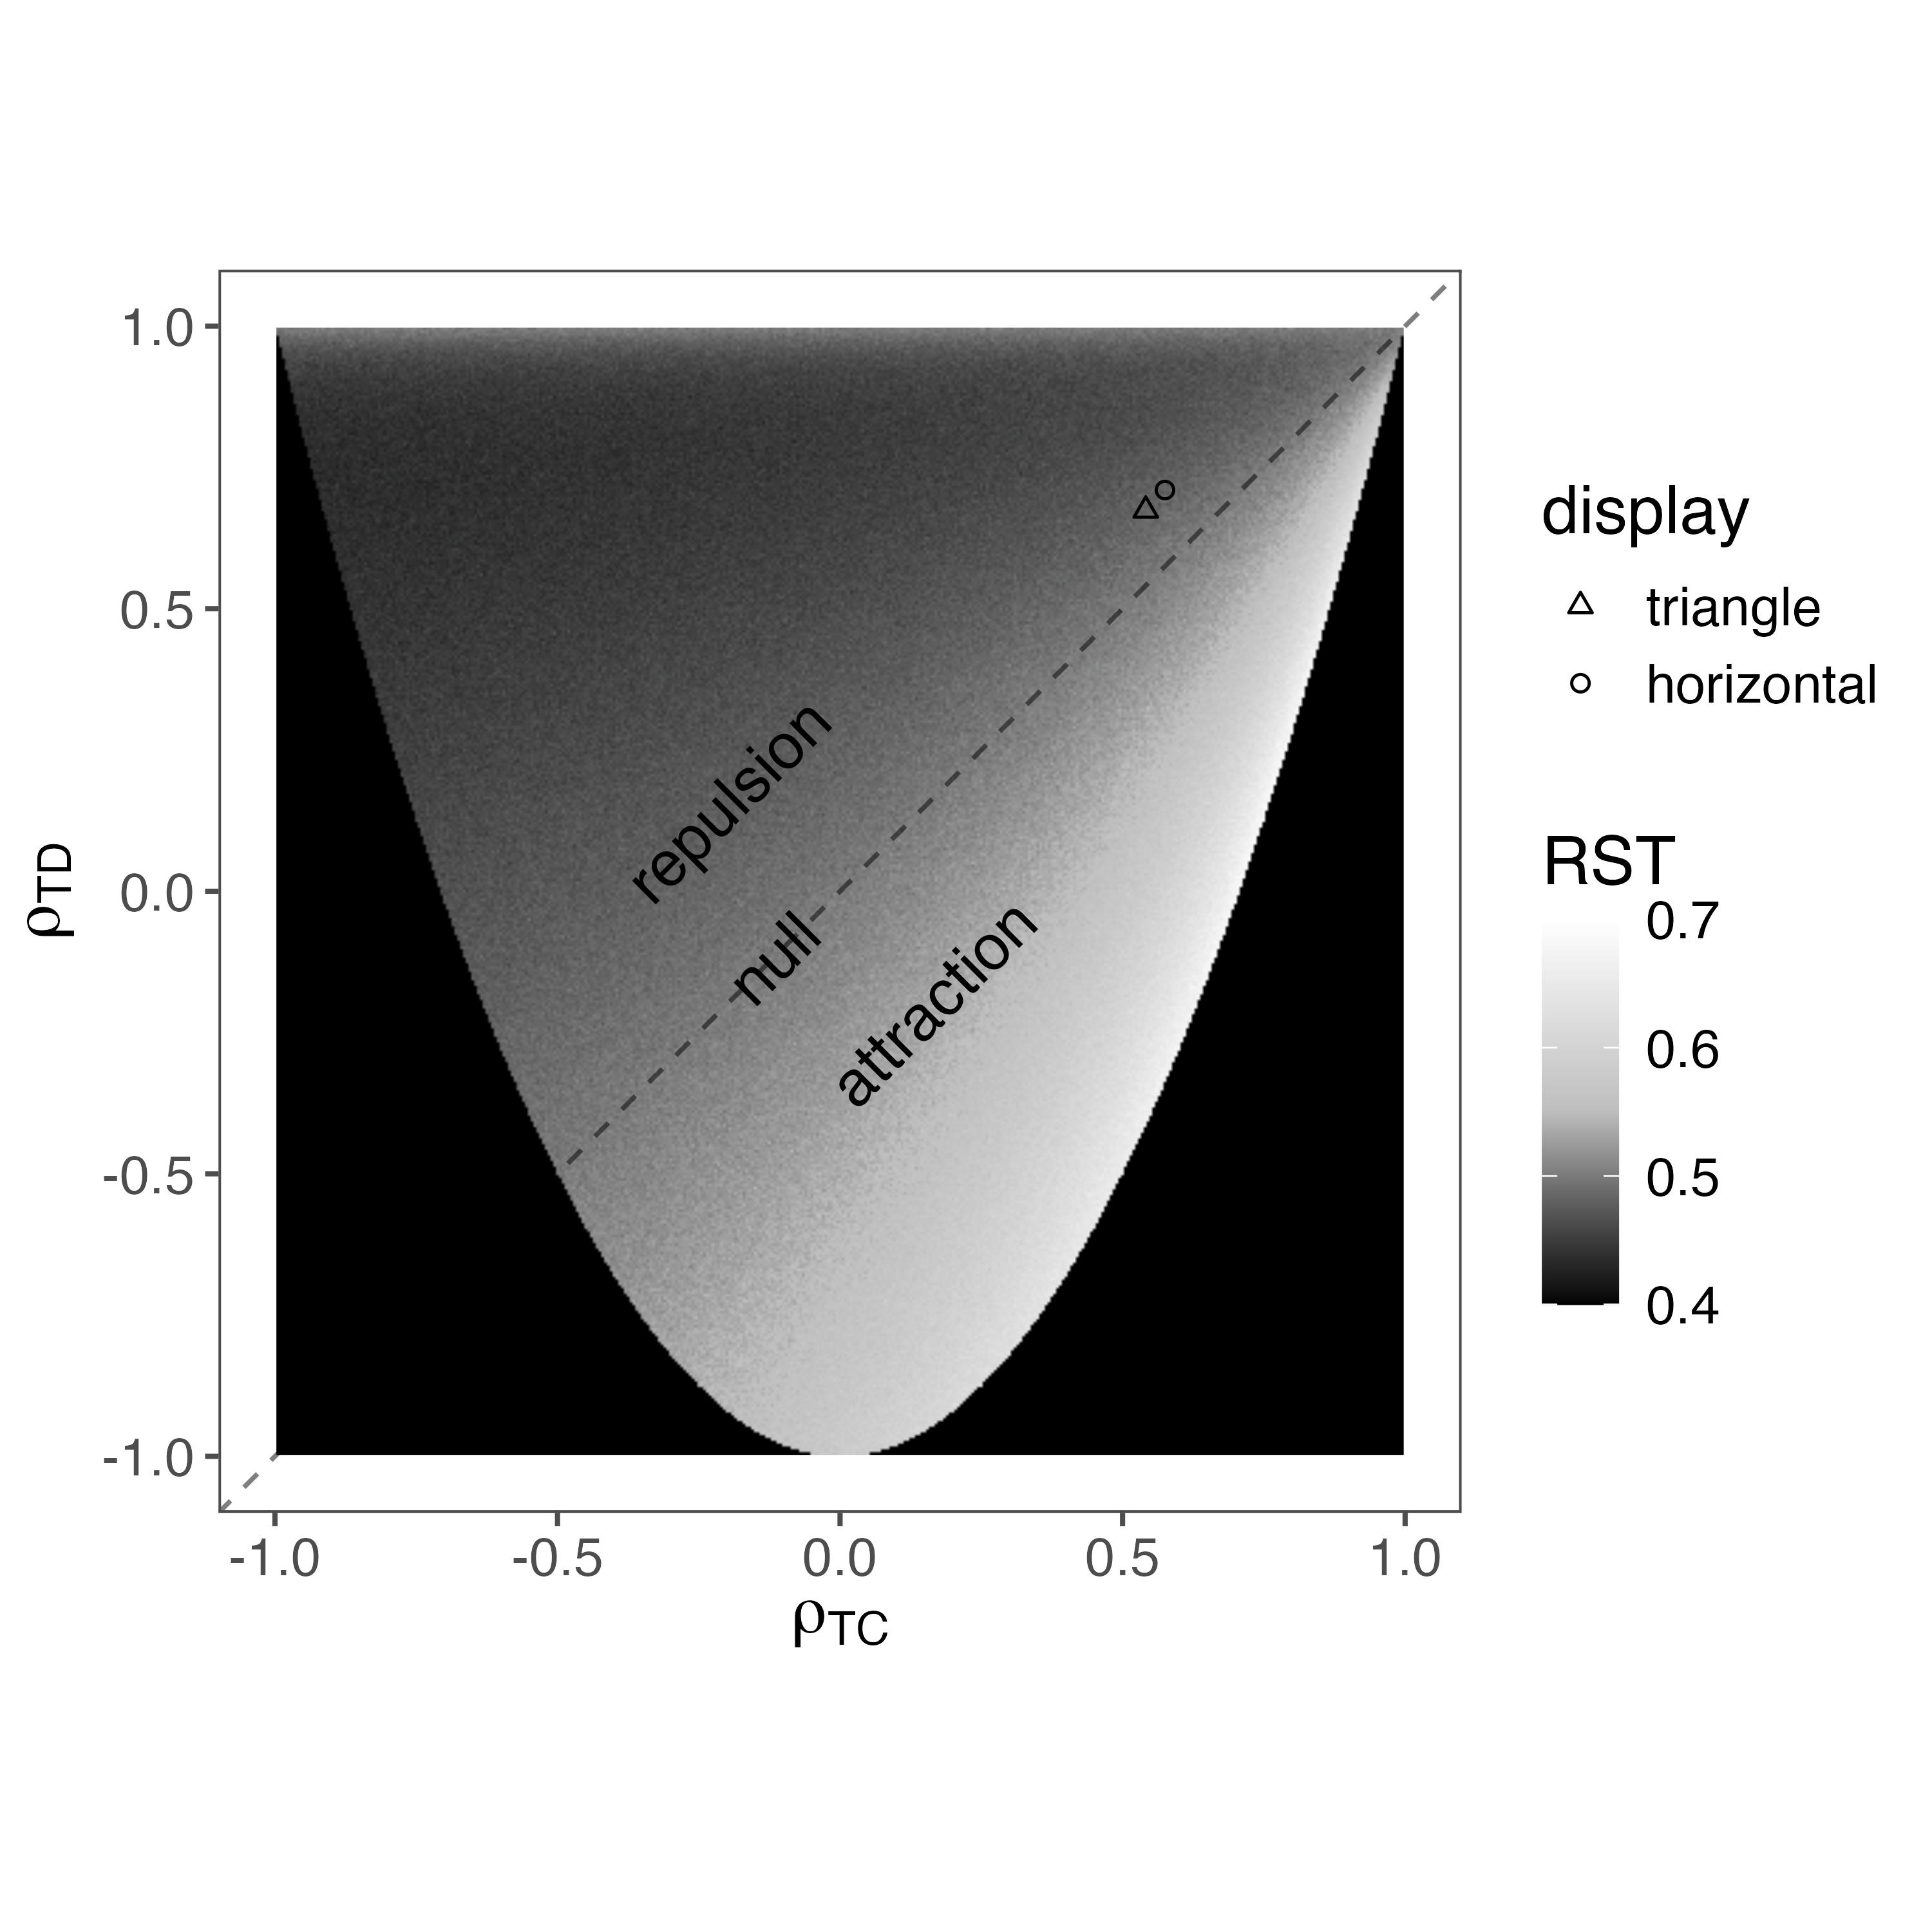
\includegraphics[width=\linewidth]{figures/3d_sim_rst.jpg}
   \caption{Model simulations for the attraction and repulsion effects based on the variation of $\rho_{TD}$ and $\rho_{TC}$. "Regions" of the plot are labeled based on their qualitative predictions for attraction, null, and repulsion effects. The black region is the area where, due to extreme correlations, a positive semi-definite variance-covariance matrix could not be formed and predictions are unavailable. The triangle and circle mark the observed mean correlations from the Experiment 2 triangle and horizontal conditions respectively.}
   \label{fig:3d_model}
\end{figure}

\subsection{Accounting for perception}
I propose that these perceptual correlations may be driving the repulsion effect in \textcite{spektorWhenGoodLooks2018b}'s data. The decoy option is smaller than the the target and competitor options and is thus not always discriminated. The triangle configuration makes discriminability particularly difficult for participants (as I show below in my Experiment 1). Simultaneously, however, the fact that target and decoy share an orientation (i.e., both wide or both tall) makes the comparison of these two options easier. In statistical terms, the perception of the decoy is more strongly correlated with the perception of the target than with perception of the competitor. Given these correlations, the perceived area of the decoy is more likely to exceed the target than the competitor. Conceptually, an empirical repulsion effect may be driven by perception rather than the "high-level" effects typically considered in the decision-making literature.

Modern psychological models of context effects often assume an attribute-wise comparison process \parencite{roeMultialternativeDecisionField2001a,trueblood2013not,usherLossAversionInhibition2004a,bhatiaAssociationsAccumulationPreference2013b}. Under this class of models, participants arrive at a decision by comparing pairs of options on a single attribute, where the modeller assumes attribute values are veridical. This assumption is quite reasonable when modeling choices where each attribute is presented separately and discriminability issues are minimal or non-existent. In this article, I present evidence that this assumption may not be appropriate. ELABORATE HERE

In Experiment 1, I first present results from a two-alternative forced-choice experiment to show that these stimuli are easily confusable and that the triangle display of \textcite{spektorWhenGoodLooks2018b} decreases discriminability relative to the triangle display. I also show that, consistent with the predictions of a perceptual model where $\rho_{TD}>\rho_{TC}>\rho_{CD}$, target-decoy discriminability is in fact \textit{easier} than competitor-decoy discriminability and that target-decoy discriminability increases with TDD. 

In Experiment 2, I combined a psychophysics task with a choice task to estimate the parameters of my perceptual model. In the first phase of the experiment, participants estimate the size of target, decoy, and competitor rectangles on each trial. In the second phase of the experiment, I conducted a standard choice experiment, replicating \textcite{spektorWhenGoodLooks2018b}'s results. I use the data from the first phase of Experiment 2 to obtain stable estimates of  $\mathbf{\mu}$ and $\mathbf{\Sigma}$ in my perceptual model. Finally, I show that the model, conditioned on the observed parameter estimates, naturally predicts a repulsion effect but not an attraction effect.  

\section{Experiment 1}

The goal of Experiment 1 was to test participants' ability to discriminate between rectangles in the perceptual choice tasks of \textcite{trueblood2013not} and \textcite{spektorWhenGoodLooks2018b}. I do, however, acknowledge the possibility that the presentation of three options (rather than just two) may impact perception. 
On each trial, I presented participants with three options (target, competitor, and decoy). After a short delay, I highlighted two of the three rectangles and asked participants to indicate which rectangle was larger. 
Additionally, I used a within-subjects manipulation to compare discriminability in both the triangle display of \textcite{spektorWhenGoodLooks2018b}, Experiment 3, and the horizontal display of \textcite{spektorWhenGoodLooks2018b}, Experiment 4a\footnote{see also \textcite{trueblood2013not}, Experiment 1.}. Otherwise, with a few exceptions discussed below, I follow the stimulus construction and experimental design of \textcite{spektorWhenGoodLooks2018b}, Experiment 3. 

\subsection{Methods}

\subsubsection{Participants.}
Data collection took place at the University of Massachusetts Amherst. 86 undergraduate students participated in exchange for course credit. 1 participant who achieved less than $80\%$ accuracy on catch trials (see below) was excluded from all analyses. Trials with response times (RTs) $<100\text{ms}$ or  $>10000\text{ms}$ were also excluded from all analyses.

\subsubsection{Stimuli.}
The experiment had two types of trials: critical trials and catch trials. 
On each critical trial, the target and competitor had the same area\footnote{Here I simplify \textcite{spektorWhenGoodLooks2018b}'s design by ensuring both focal stimuli had the same area.} but differed on orientation, with one stimulus being wide and the other tall. The decoy always had the same orientation as the target. The height and width of the decoy were reduced proportionally so that the decoy area was always $0\%$, $2\%$, $5\%$, $9\%$, or $14\%$ of the target areas. Because the target and competitor always had the same area, this means that the decoy was also $0\%$, $2\%$, $5\%$, $9\%$, or $14\%$ of the competitor area. These are the TDD values from \textcite{spektorWhenGoodLooks2018b}, plus a $0\%$ level which acted as a baseline\footnote{When TDD=$0\%$, the target and decoy are identical, so labeling is arbitrary.}.

\subsubsection{Design.}
There were 5 blocks of trials. In each block there were 60 critical trials, 12 at each TDD level, and 30 catch trials. Of the 12 critical trials at each TDD level, 6 were presented in a triangle and 6 were presented horizontally. Finally, 3 of the 6 targets in each display condition at each TDD level were wide and 3 were tall. Of each of these 3, one was a target-decoy comparison, one was a target-competitor comparison, and one was a target-competitor comparison. Trial order and rectangle order within each trial were randomized.

On each catch trial, there was one large rectangle and two much smaller rectangles. The large rectangle was $260 \pm U(-40, 40) \text{x} 200 \pm U(-40, 40)$ pixels, with a random orientation. The smaller rectangles were $180 \pm U(-40, 40) \text{x} 120 \pm U(-40, 40)$ pixels, one wide and one tall.

On every trial, the rectangles were displayed in either a triangle or horizontal display (see \ref{fig:spektor_stim}). The horizontal distance between all rectangles was constant, but 25 pixels of jitter was added to each rectangle's vertical location.

Stimuli were presented on computer monitors with a resolution of 1920 x 1080 pixels. The experiment was programmed with jsPsych \parencite{deleeuwJsPsychJavaScriptLibrary2015}. 

\subsubsection{Procedure.}
On each trial, participants saw three rectangles, labeled 1, 2, and 3 (from left to right). The rectangles appeared for 1825ms total, but after 500ms, two of the rectangles changed to a darker shade. After all three rectangles disappeared from the screen, participants were asked to select which of the two darker rectangles had the larger area.

\subsection{Results}

\subsubsection{Catch Trials.}
Participants performed well on the catch trials. The mean percentage correct in the triangle display was $92.6\% (SD=3.77)$, and the mean percentage correct in the triangle display was $93.2\% (SD=3.52)$. 

\subsubsection{Critical Trials.}
I first checked the baseline TDD level data (TDD=$0\%$) across to make sure that participants were indifferent between pairs of options when they had identical area. The mean percentage of target choices in target-competitor trials was $48.99\%$ (SD=10.18). The mean percentage of competitor choices in competitor-decoy trials was $49.80\%$ (SD=11.30). The mean percentage of target choices in target-decoy trials was $49.47\%$ (SD=12.06). Participants were indifferent between all pairs of options in the $\text{TDD}=0\%$ trials, so I do not consider these trials further.

The primary analysis was performed on the target-decoy and competitor-decoy trials, excluding the TDD=$0\%$ trials. In these trials participants' task is simply to not select the decoy option on a given trial. I present mean choice proportions across conditions in Figure \ref{fig:e1_data}. Participants' performance indeed improves with TDD. Furthermore, their performance is better when stimuli are displayed in the horizontal configuration than in the triangle configuration, and it is also better in target-decoy trials compared to competitor-decoy trials. Finally, there is an interaction, such that as TDD increases, the target-decoy performance is even better than the competitor-decoy performance. See Appendix XXX for inferential statistics which support these conclusions.

\begin{figure}
   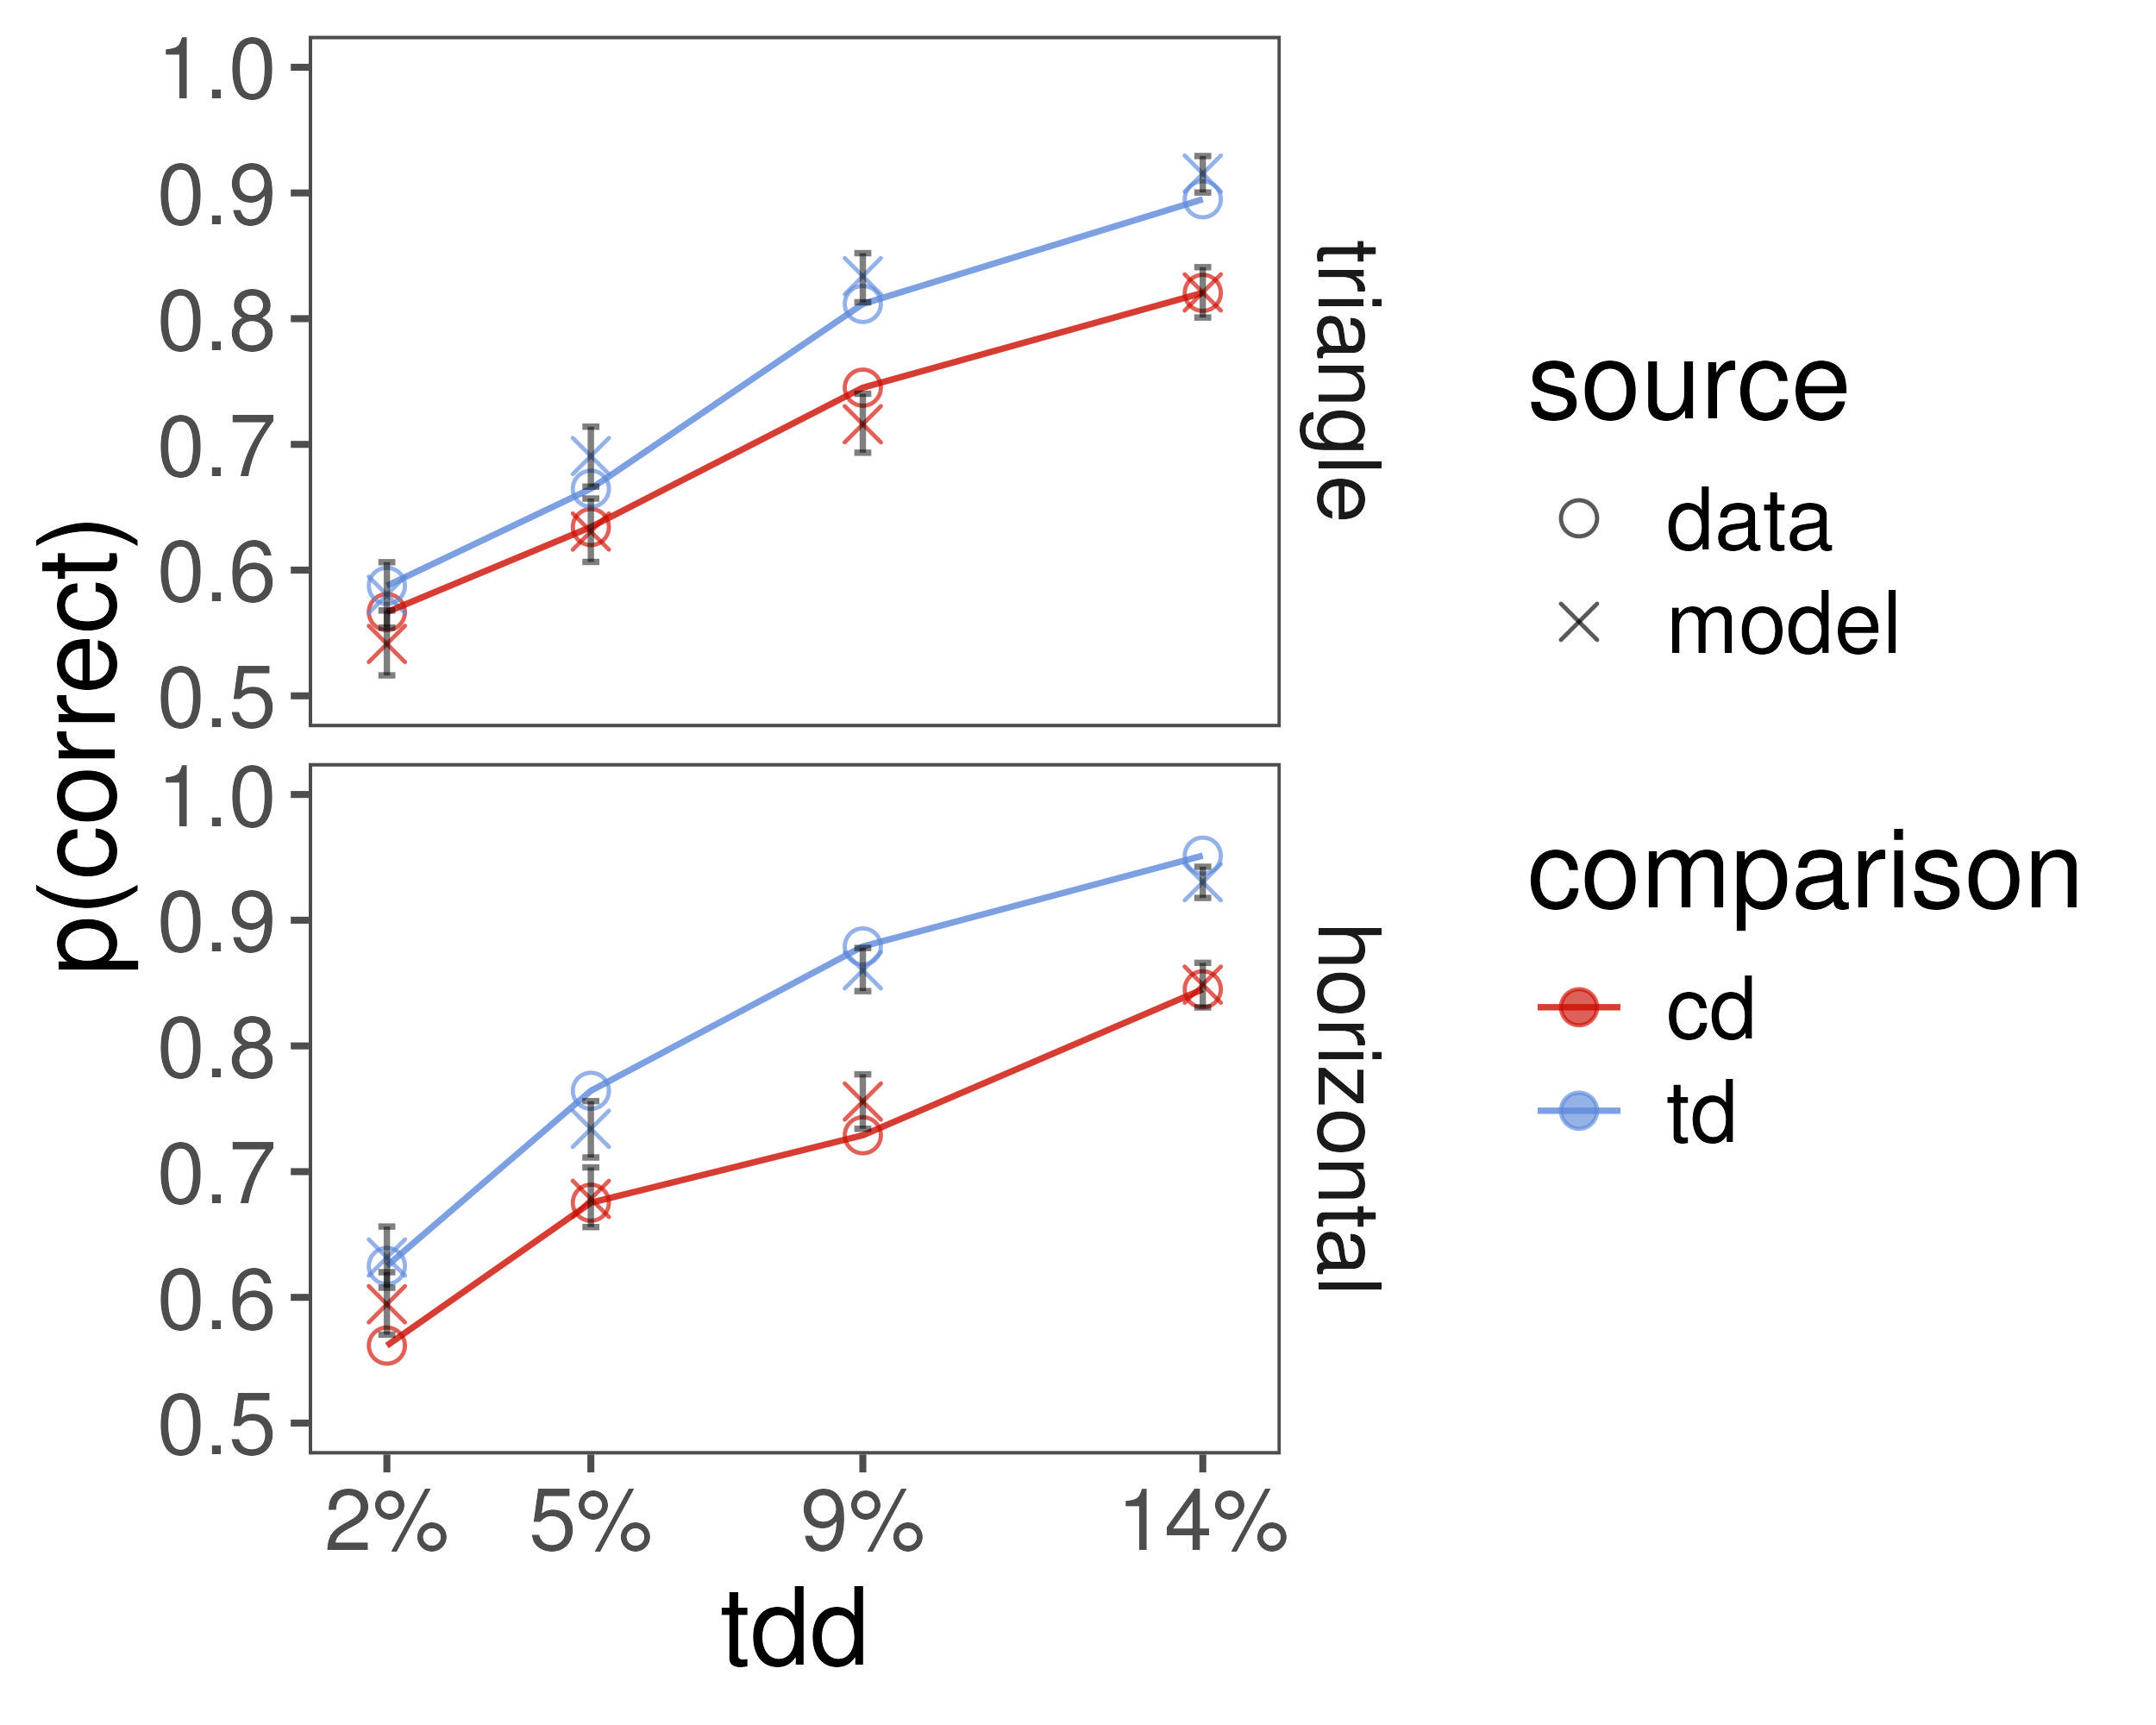
\includegraphics[width=\textwidth]{figures/m13_model_preds_v_data.jpeg}
   \caption{Experiment 1, mean choice proportions by stimulus display, TDD, and comparison. td=target-decoy trials, dc=competitor-decoy trials. Model predictions come from the Bayesian hierarchical logistic regression presented in Appendix XXX. Error bars are $95\%$ HDIs on the mean.}
   \label{fig:e1_data}
\end{figure}

\subsubsection{Discussion}
In Experiment 1, I showed that participants are not always able to discriminate between target-decoy and competitor-decoy stimuli. I also show that this discriminability increases with TDD and that overall discriminability is better in the horizontal compared to the triangle display. Finally, through the interaction of comparison-pair and TDD, I show that target-decoy discriminability increases with TDD at a higher rate than competitor-decoy discriminability. 

These results, in fact, are natually predicted by a model where $\rho_{TD}>\rho_{CD}$ (see Appendix XXX for simulations - NEED TO DO THIS).

\section{Experiment 2}
I continue this line of research in Experiment 2, where I used a psychophysics task to estimate the mean perceived area and correlations between perceived area to the target, competitor, and decoy rectangles. Experiment 2 used the \textit{method of cross-modal matching} \parencite{stevensCrossmodalityMatchingBrightness1965}, where participants adjusted the size of a circle to match the perceived area for each rectangle. On each trial, participants saw three rectangles and three circles, each labeled 1, 2, and 3. Participants adjusted the size of the circle corresponding to each rectangle, until they believed the two to have equal area. I also replicate \textcite{spektorWhenGoodLooks2018b}'s choice data in a second phase of the experiment. Finally, I used a between-subjects manipulation to display the rectangle stimuli in either the horizontal or triangle displays of \textcite{spektorWhenGoodLooks2018b}.

\subsubsection{Methods}
\subsubsubsection{Participants.}
Data collection took place at the University of Massachusetts Amherst. 521 undergraduate students participated in exchange for course credit. 68 participants did not complete the full experiment within the 1 hour time limit and were removed from all analyses. 

\subsubsubsection{Stimuli.}
In the circle adjustment phase there were three types of trials: critical trials, filler trials, and catch trials. On each critical trial, the target and competitor had the same area but differed on orientation, with one stimulus being wide and the other tall. The decoy always had the same orientation as the target. I varied TDD at $2\%$, $5\%$, $9\%$, and $14\%$. I also varied the target, competitor, and decoy stimuli to fall on three diagonals. In pixels, the small and larger focal stimulus dimension values on the lower, middle, and upper diagonals were $[60, 135]$, $[90, 165]$, and $[120,195]$. I reduced the absolute size of the target/competitor stimuli from Experiment 1 to Experiment 2 to accomodate the circle adjustment phase (see procedure  below).

On filler trials, I randomly sampled three rectangles by sampling a height and width from the distribution $U(56,195)$, encompassing the full range of stimuli from the critical trials.

On the catch trials, I randomly sampled one rectangle from the lower diagonal and two from the upper diagonal, so one stimulus was clearly larger than the other two.

The choice phase had identical trial types with the exception that there were no catch trials, only critical and filler trials.

\subsubsubsection{Design.}
Across both phases, I varied display condition between-subjects and TDD, diagonal, target-decoy orientation within-subjects. After removing subjects, there were 218 participants in the horizontal display condition and 225 participants in the triangle display condition. 

In the circle adjustment phase, there were 4 blocks, each 40 trials. Each block consisted of 24 critical trials, 14 filler trials, and 2 catch trials. Within the critical trials, there were 6 trials at each level of TDD. In 3 of these 6 trials the target and decoy were oriented wide (choice set $[w,h,d_{w}]$), and in the other 3 target and decoy were oriented tall (choice set $[w,h,d_{h}]$). 

In the choice phase, there were 4 blocks, each with 34 trials. 24 of these trials were critical trials and 10 were filler trials. Of these 24 critical trials, there were 6 trials at each level of TDD. Within each 6, there were 3 trials where target and decoy were oriented wide and 3 were target and decoy were oriented tall. 

\subsubsubsection{Procedure.}

The experiment took place in two phases: 

On each circle adjustment trial, three gray rectangles appeared in the lower left corner of the screen, either in a triangle or horizontal display. In the upper right, three gray circles appeared in the upper right of the screen, in the same display as the rectangles (see Figure \ref{fig:circle_exp_display} ). A small amount of jitter ($U(-15,15)\text{px}$) was added to the position of each rectangle and the corresponding circle. Each circle started with an area of 78 square pixels (i.e., with a radius of 5), the minimum size I allowed in the experiment. Participants used the mouse to adjust the circle. Within a single trial, they were free to adjust the circles in any order they liked or to go re-adjust a circle as much as they liked. There was no time limit to each adjustment trial. The maximum circle area allowed was 65144 square pixels\footnote{I arrive at this number based on the maximum area the circles could be while only appearing on the right half of the screen and maintaining the same horizontal distance from each other as the corresponding rectangles.}. When a participant finished adjusting the circles on a trial, they clicked the "Submit" button located on the lower right hand corner of the screen. 

The circle adjustment phase began with three practice trials, followed by the 4 blocks of experimental trials. At the beginning of each experimental block, participants completed 3 calibration trials. Calibration trials were identical to filler trials, with the caveat that I provided feedback after participants' responses. After participants submitted their responses on a trial, a red circle appeared around each adjusted circle, showing the true area of the corresponding rectangle. 

Throughout the circle phase, I kept track of the deviations between the true rectangle areas and the participants' adjusted circle areas. At the end of each block, I computed the current mean deviation, and, depending on this value, told the participant that they were either over or under-adjusting, on average.

The choice phase began with 3 practice trials. Participants were not provided feedback during these practice trials. 

On each choice trial, three rectangles appeared in the center of the screen in a horizontal or triangle display. There was no vertical jitter added here. Participants were told to select the rectangle with the largest area by clicking on it.

At the end of the choice phase, I let each participant know their percentage correct from the choice phase. Note that in a critical trial, a correct response is simply one where they did not select the decoy, as the target and competitor rectangles always had the same area.

Stimuli were presented on computer monitors with a resolution of 1920 x 1080 pixels. The experiment was programmed with GNU Octave \parencite{octave} and PsychoPhysics Toolbox \parencite{brainardPsychophysicsToolbox1997}. 

\begin{figure}
   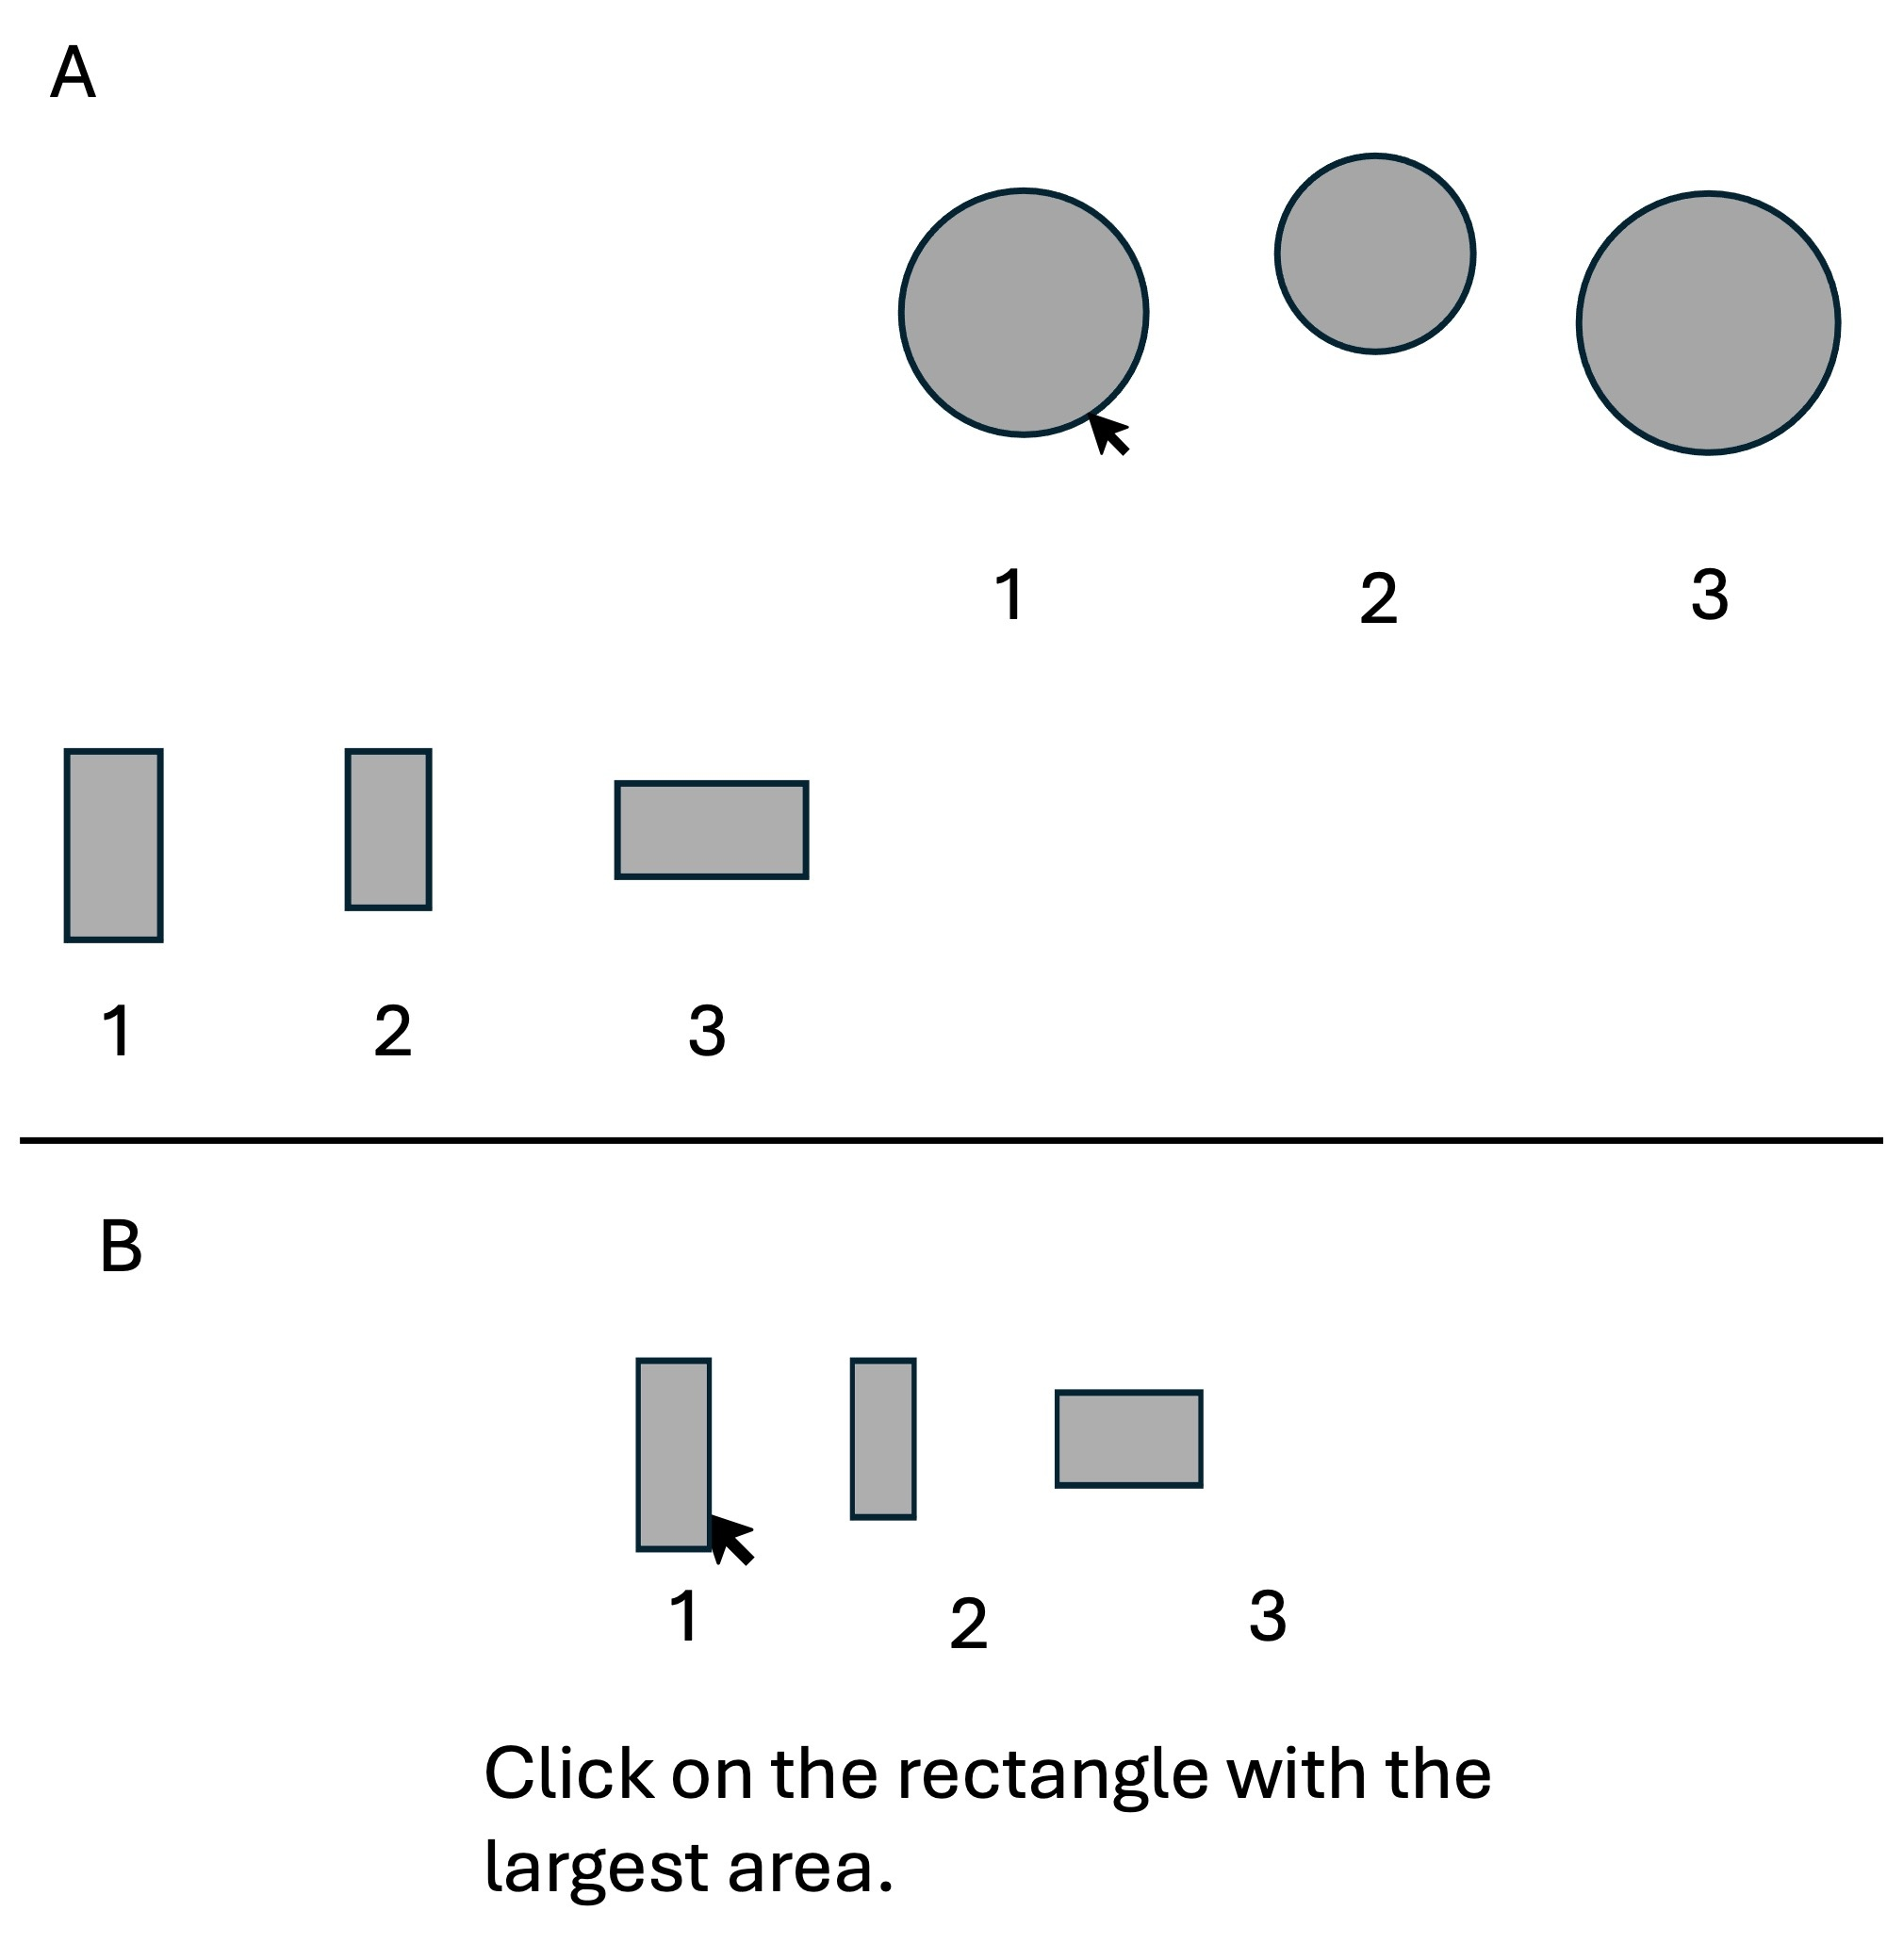
\includegraphics[width=\linewidth]{figures/circle_exp_display.jpg}
   \caption{Example trials from Experiment 2. A: Circle adjustment phase. B: Choice phase. This an example of trials in the horizontal display condition.}
   \label{fig:circle_exp_display}
\end{figure}

\subsubsection{Results}
\subsubsubsection{Data Processing}
Given the difficulty of the circle adjustment task, the data required processing to ensure that outlier trials and participants did not influence our estimates of $\mathbf{Omega}$.

First, I removed all participants who did not give correct responses on $75\%$ ($6/8)$ of the catch trials. A correct response entails estimating the larger rectangle to be the largest on the trial. 10 participants were removed from all analyses after they failed to achieve at least $75\%$ correct on catch trials (see below for details). This left a total of 443 participants.

Next, from the remaining participants, I first natural log-transformed all responses. I then dropped all trials where at least one circle was not adjusted (i.e., at least one circle was left at the starting size).

I then removed outlier participants using the following procedure:

I fit a linear regression to each individual participants' data, regressing each log circle area on each corresponding log rectangle area. I then computed an $R^2$ for each participant. I then removed all participants whose $R^2$ fell below the $5\%$ quantile for all $R^2$s, which in this case was $.3975$. This removed 23 subjects, leaving us with a total of 420 participants, 213 in the triangle display condition and 207 in the horizontal display condition. Of the remaining participants, $R^2$ values were high ($M=.67,SD=.12$), indicating they could generally perform the task.

From the $420$ partipants whose data I analyzed, I removed outlier trials from the critical trial data. I did so to ensure that any outliers do not influence our estimates of $\rho_{TD}$, $\rho_{TC}$, or $\rho_{CD}$. I z-transformed all log circle areas within each participant and diagonal. I remove all critical trials where at least one z-score had an absolute value above $3.5$. This led to $102$ trials being dropped. I dropped $0$, $1$, $2$, and $4$ critical trials from $339$, $62$, $18$, and $1$ participants, respectively. 

After all circle phase data processing, I were left with $20371$ trials in the triangle display condition and $19809$ trials in the horizontal display condition. 

For the choice phase, I only retained participants whose data I retained in the circle phase.

\subsubsubsection{Circle Phase Results - Critical Trials}
Before modeling our data, I wanted to ensure that participants could successfully perform the task. While I do not expect perfect performance in an absolute sense, I do require adequate relative performance. 

To assess performance on the critical trials, I computed the mean difference between actual log area and estimated log area for each subject, stimulus pair (i.e., target-competitor, target-decoy, competitor-decoy), and actual difference. I plot these via a set of boxplots in Figure \ref{fig:circle_boxplots}. Although participants vary considerably in their judgments, I find that on average, participants' adjusted circle areas increase with the absolute size of rectangles. 


\begin{figure}
   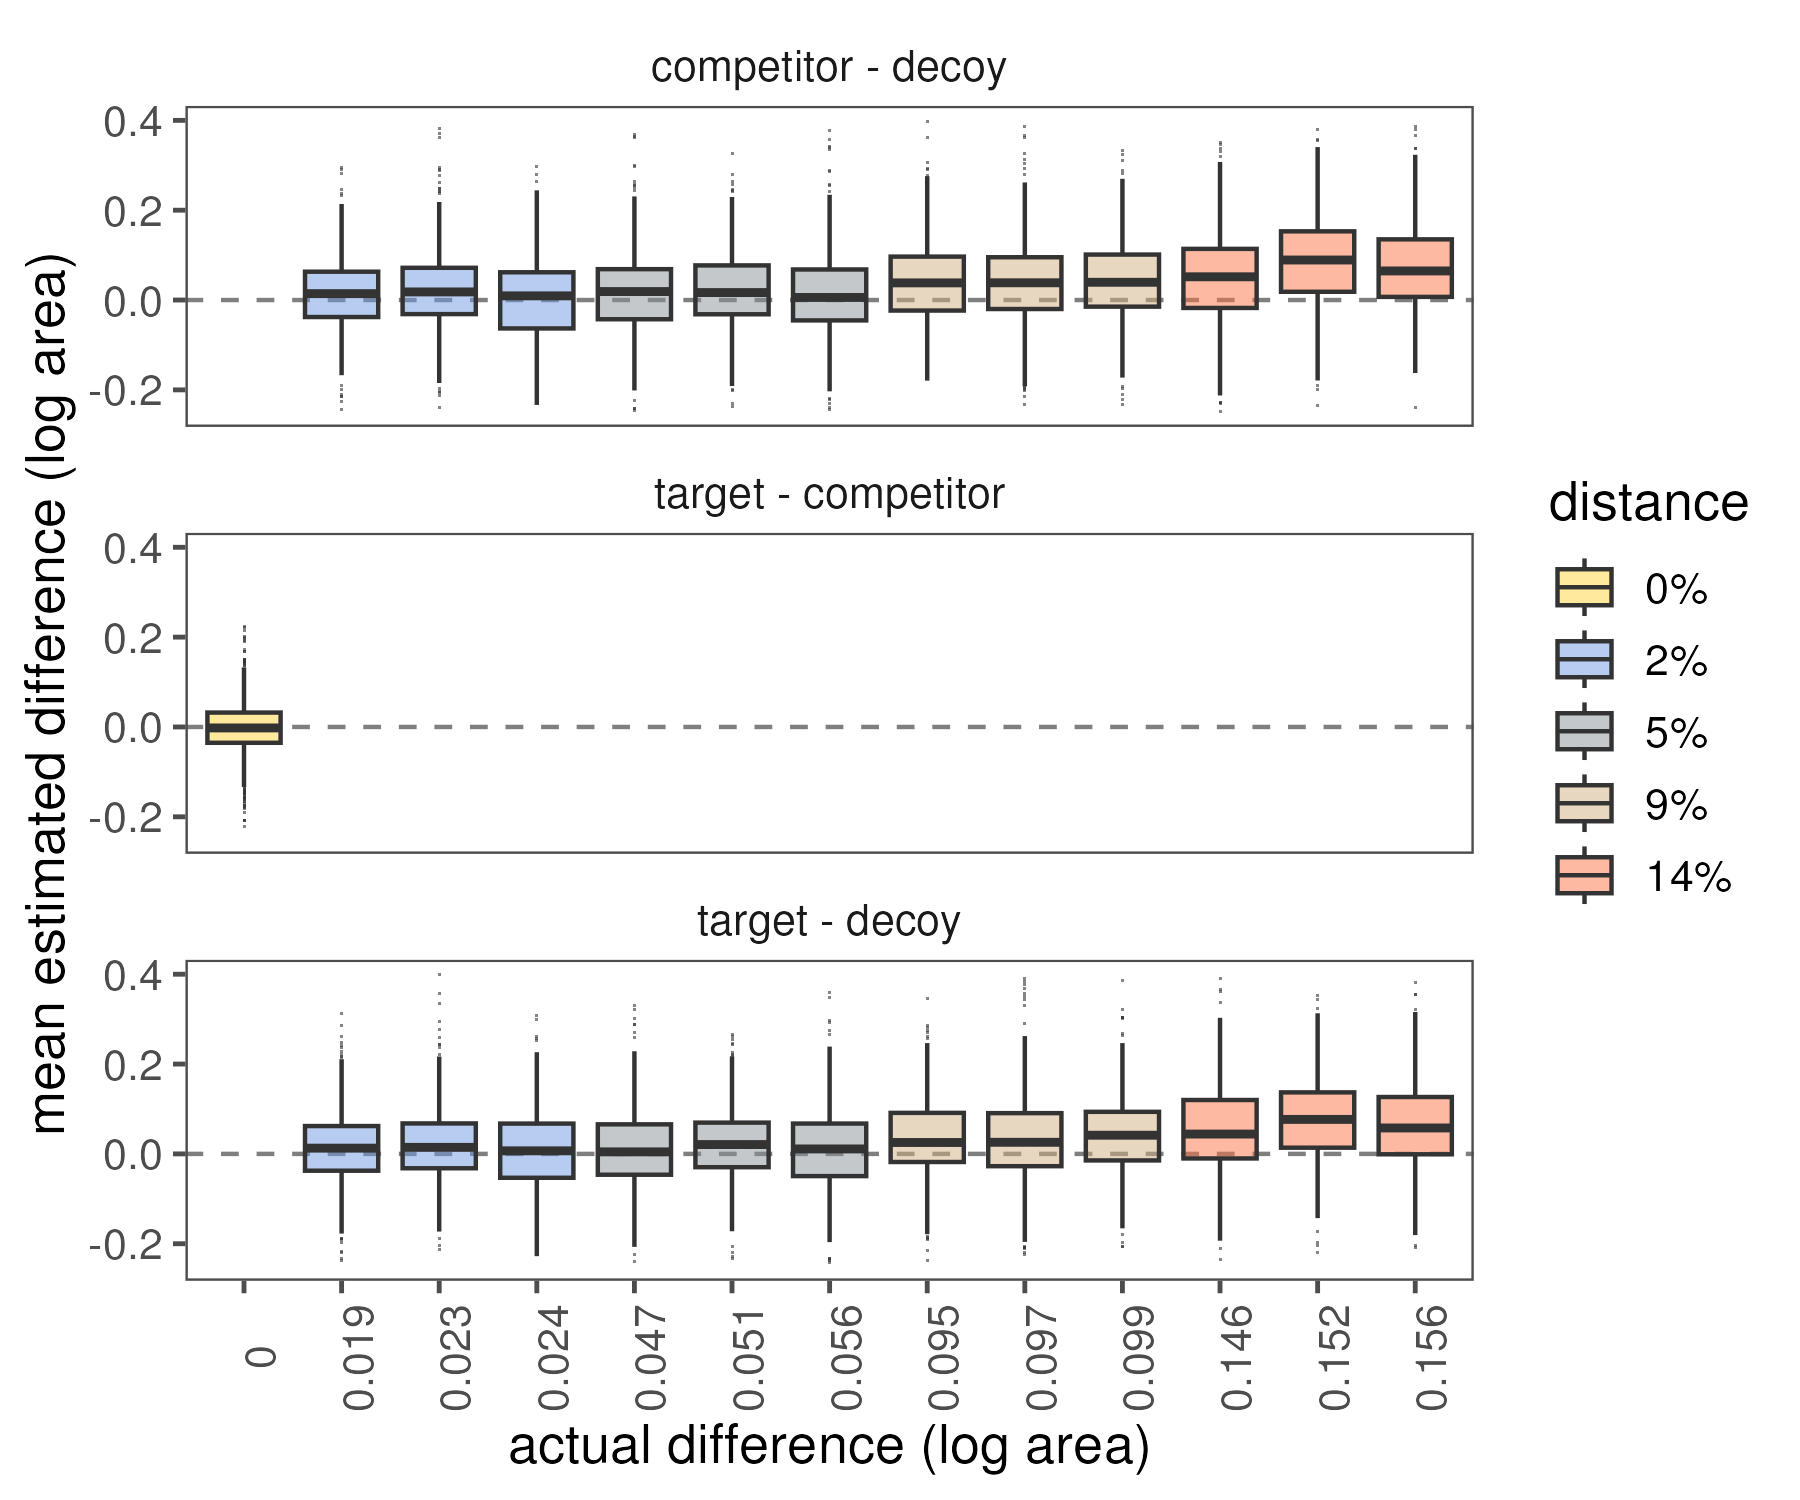
\includegraphics[width=\textwidth]{figures/circleAreaPhase_boxplot_meanlogdiffs_no_outliers.jpeg}
   \caption{Boxplot of subject-level mean error in area estimations, split by stimulus pair, TDD, and absolute discrepancy in rectangle area. Note that because the target and competitor rectangles always had equal areas, the true difference is always 0.}
   \label{fig:circle_boxplots}
\end{figure}

I next present scatterplots of all pairwise circle areas from each trial, see Figure \ref{fig:raw_cors}. I present these to be transparent about the raw data and to illustrate the necessity of a statistical model to understand these correlations. 

\begin{figure}
   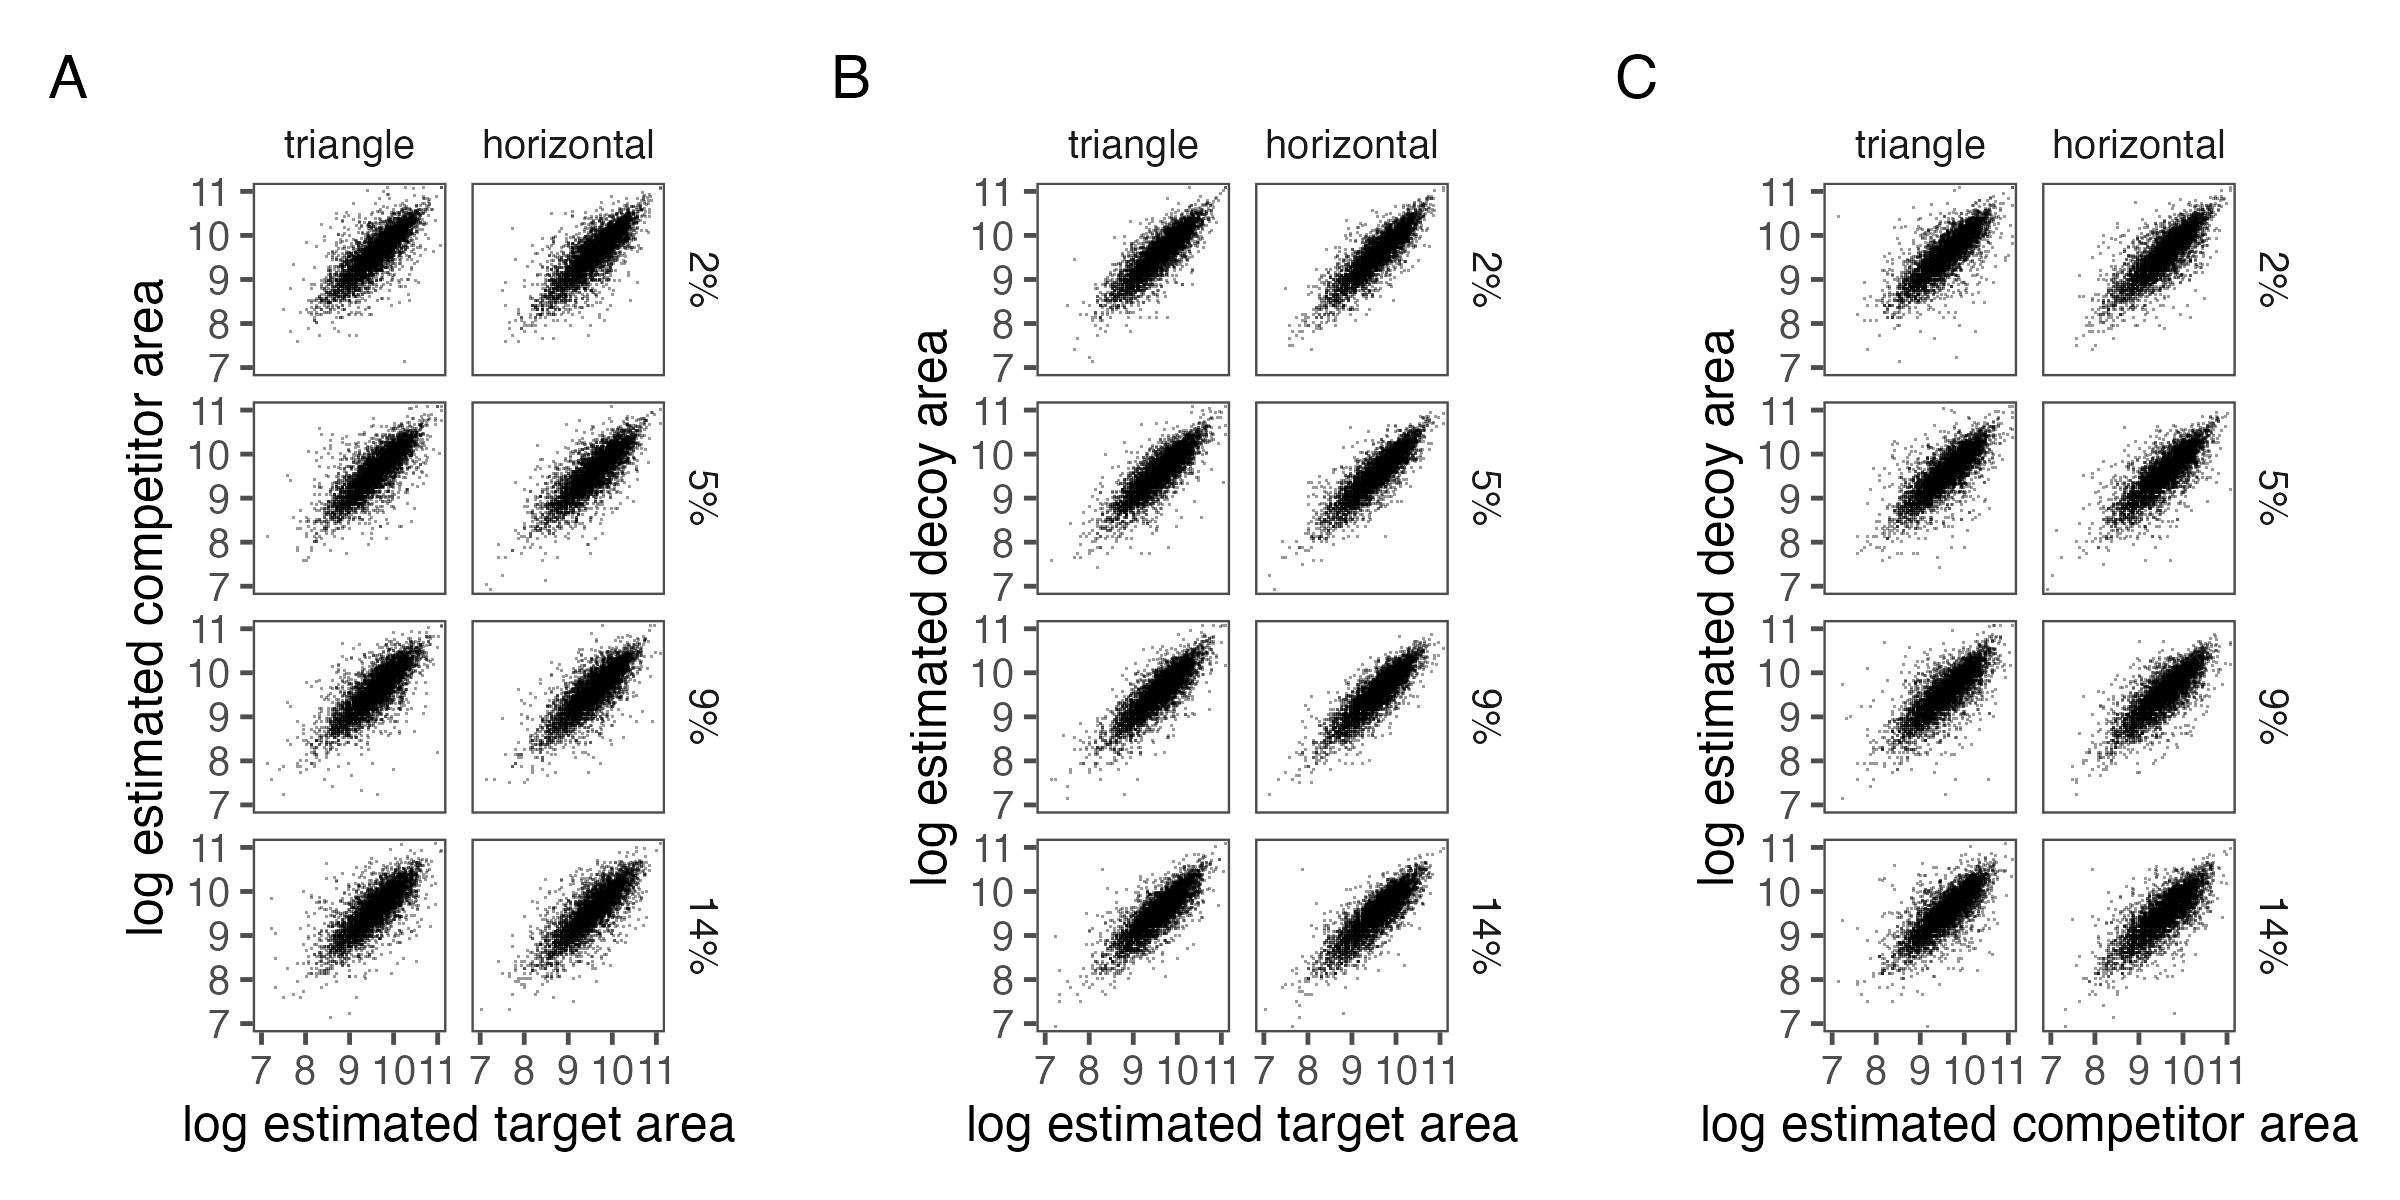
\includegraphics[width=\textwidth]{figures/circleAreaPhase_cor_plot_all_no_outliers.jpg}
   \caption{Scatterplots of target-competitor (A), target-decoy (B), and competitor-decoy (C) correlations, split by display condition and TDD.}
   \label{fig:raw_cors}
\end{figure}

Computing raw correlations, without accounting for subject and trial-level differences, will grossly inflate the size of these correlations. Moreover, any differences between, say, $\rho_{TD}$ and $\rho_{CD}$ are bound to be small. I used Bayesian hierarchical modeling to estimate the parameters of a multivariate normal distribution (as outlined in the introduction), with parameters $\mathbf{\mu}$ and $\mathbf{\sigma}$. I present the details of the model in Appendix XXX but present the main results below.

I assume that, for participant $i$, on each critical trial $j$, the perceived target, competitor, and decoy areas $X_{i}$ are sampled from a multivariate normal distribution with mean vector $\mathbf{\mu_{ij}$ and variance-covariance matrix $\mathbf{\Sigma}$. 

As discussed in the Introduction, I decompose sigma into the $S\mathbf{\Omega}S$, where the diagonal elements of $S$ are population standard deviations and the off diagonal elements are $0$. $\Omega$ is $3x3$ correlation matrix.  

I focus on our estimates of $\mathbf{\mu$ and $\Omega$ in the main text and discuss the details of the modeling, along with $\S$ estimates, in Appendix XXX. 

I show mean estimates of $\mathbf{\mu}$ in Figure \ref{fig:e2mu} and show estimates of $\mathbf{\Omega}$ in Figure \ref{fig:omega}. In both conditions, $\rho_{TD}$ is larger than both $\rho_{CD}$ and $\rho_{TC}$, while $\rho_{CD}$ and $\rho_{TC}$ do not differ from each other. 

\begin{figure}
   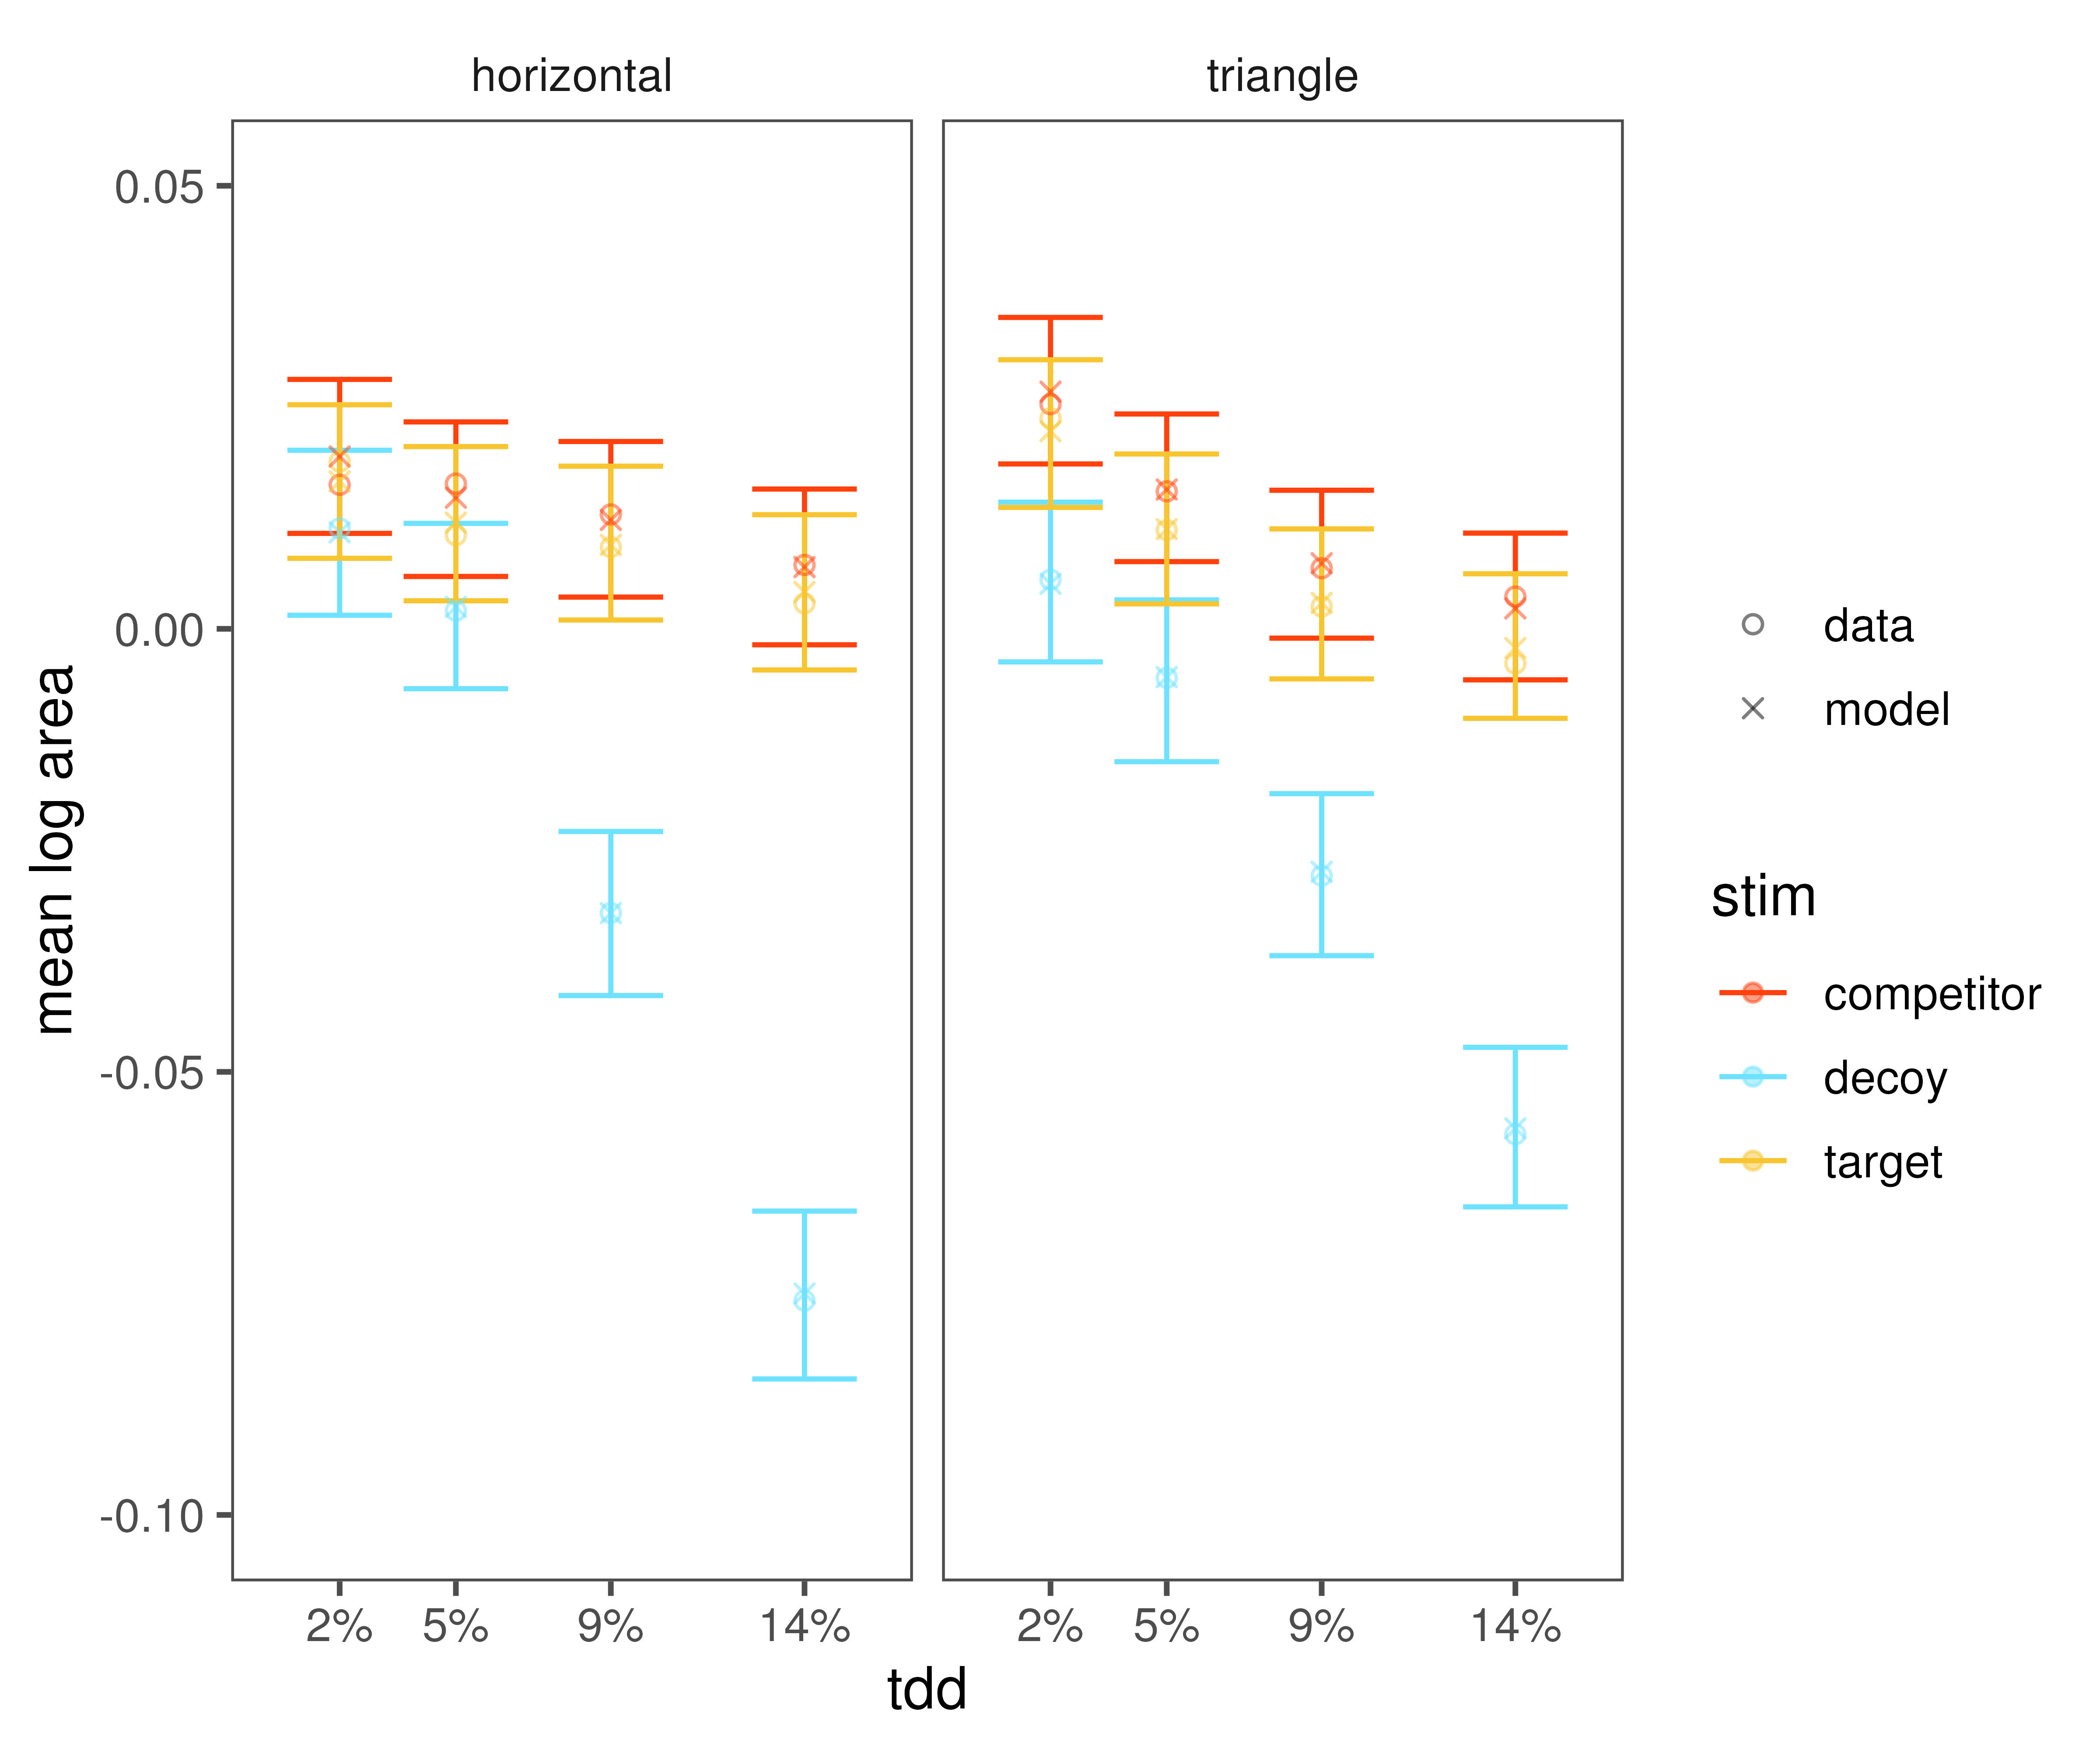
\includegraphics[width=\textwidth]{figures/bayes_circle_area_mu_sigma_constant_comp_effect_model_v_data_collapsed.jpeg}
   \caption{$\mathbf{\mu$ estimates from Experiment 2.}
   \label{fig:e2mu}
\end{figure}

\begin{figure}
   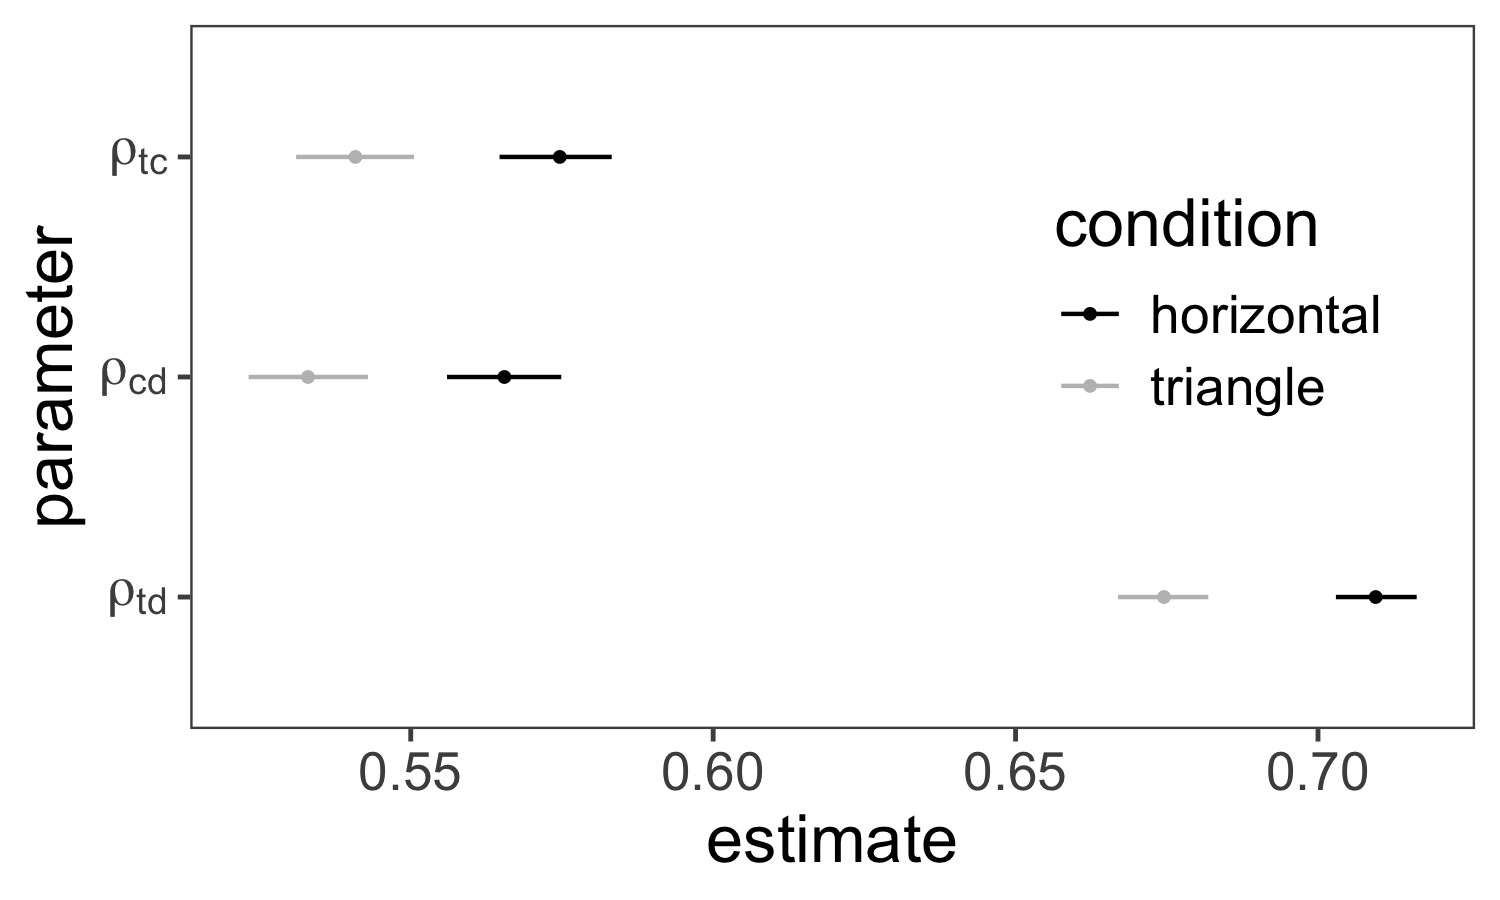
\includegraphics[width=\textwidth]{figures/bayes_circle_area_sigma_constant_comp_effect_omega_plot.jpeg}
   \caption{Posterior estimate of $\Omega$ (off-diagonal parameters) across display conditions. Lines show $95\%$ HDIs.  Dots indicate means.}
   \label{fig:omega}
\end{figure}

\subsubsubsection{Choice Results}

I present mean choice proportions across display conditions and TDD in figure \ref{fig:e2_choiceprops}. I replicate the qualitative results of \textcite{spektorWhenGoodLooks2018b}. At low levels of TDD, I find a repulsion effect in both display conditions. At higher levels of TDD, I either find a null effect (triangle condition) or an attraction effect (horizontal condition). 

To ensure that this result is not an artifact of averaging across choice sets, I present mean changes in choice proportion for the options $w$ and $h$ across the two choice sets $[w,h,d_{w}]$ and $[w,h,d_{h}]$ (see \ref{fig:e2_choicedeltas}). These results also show that low levels of TDD create a repulsion effect, while higher levels create a null or attraction effect. See Appendix XXX for inferential statistics that support these conclusions.

\begin{figure}
   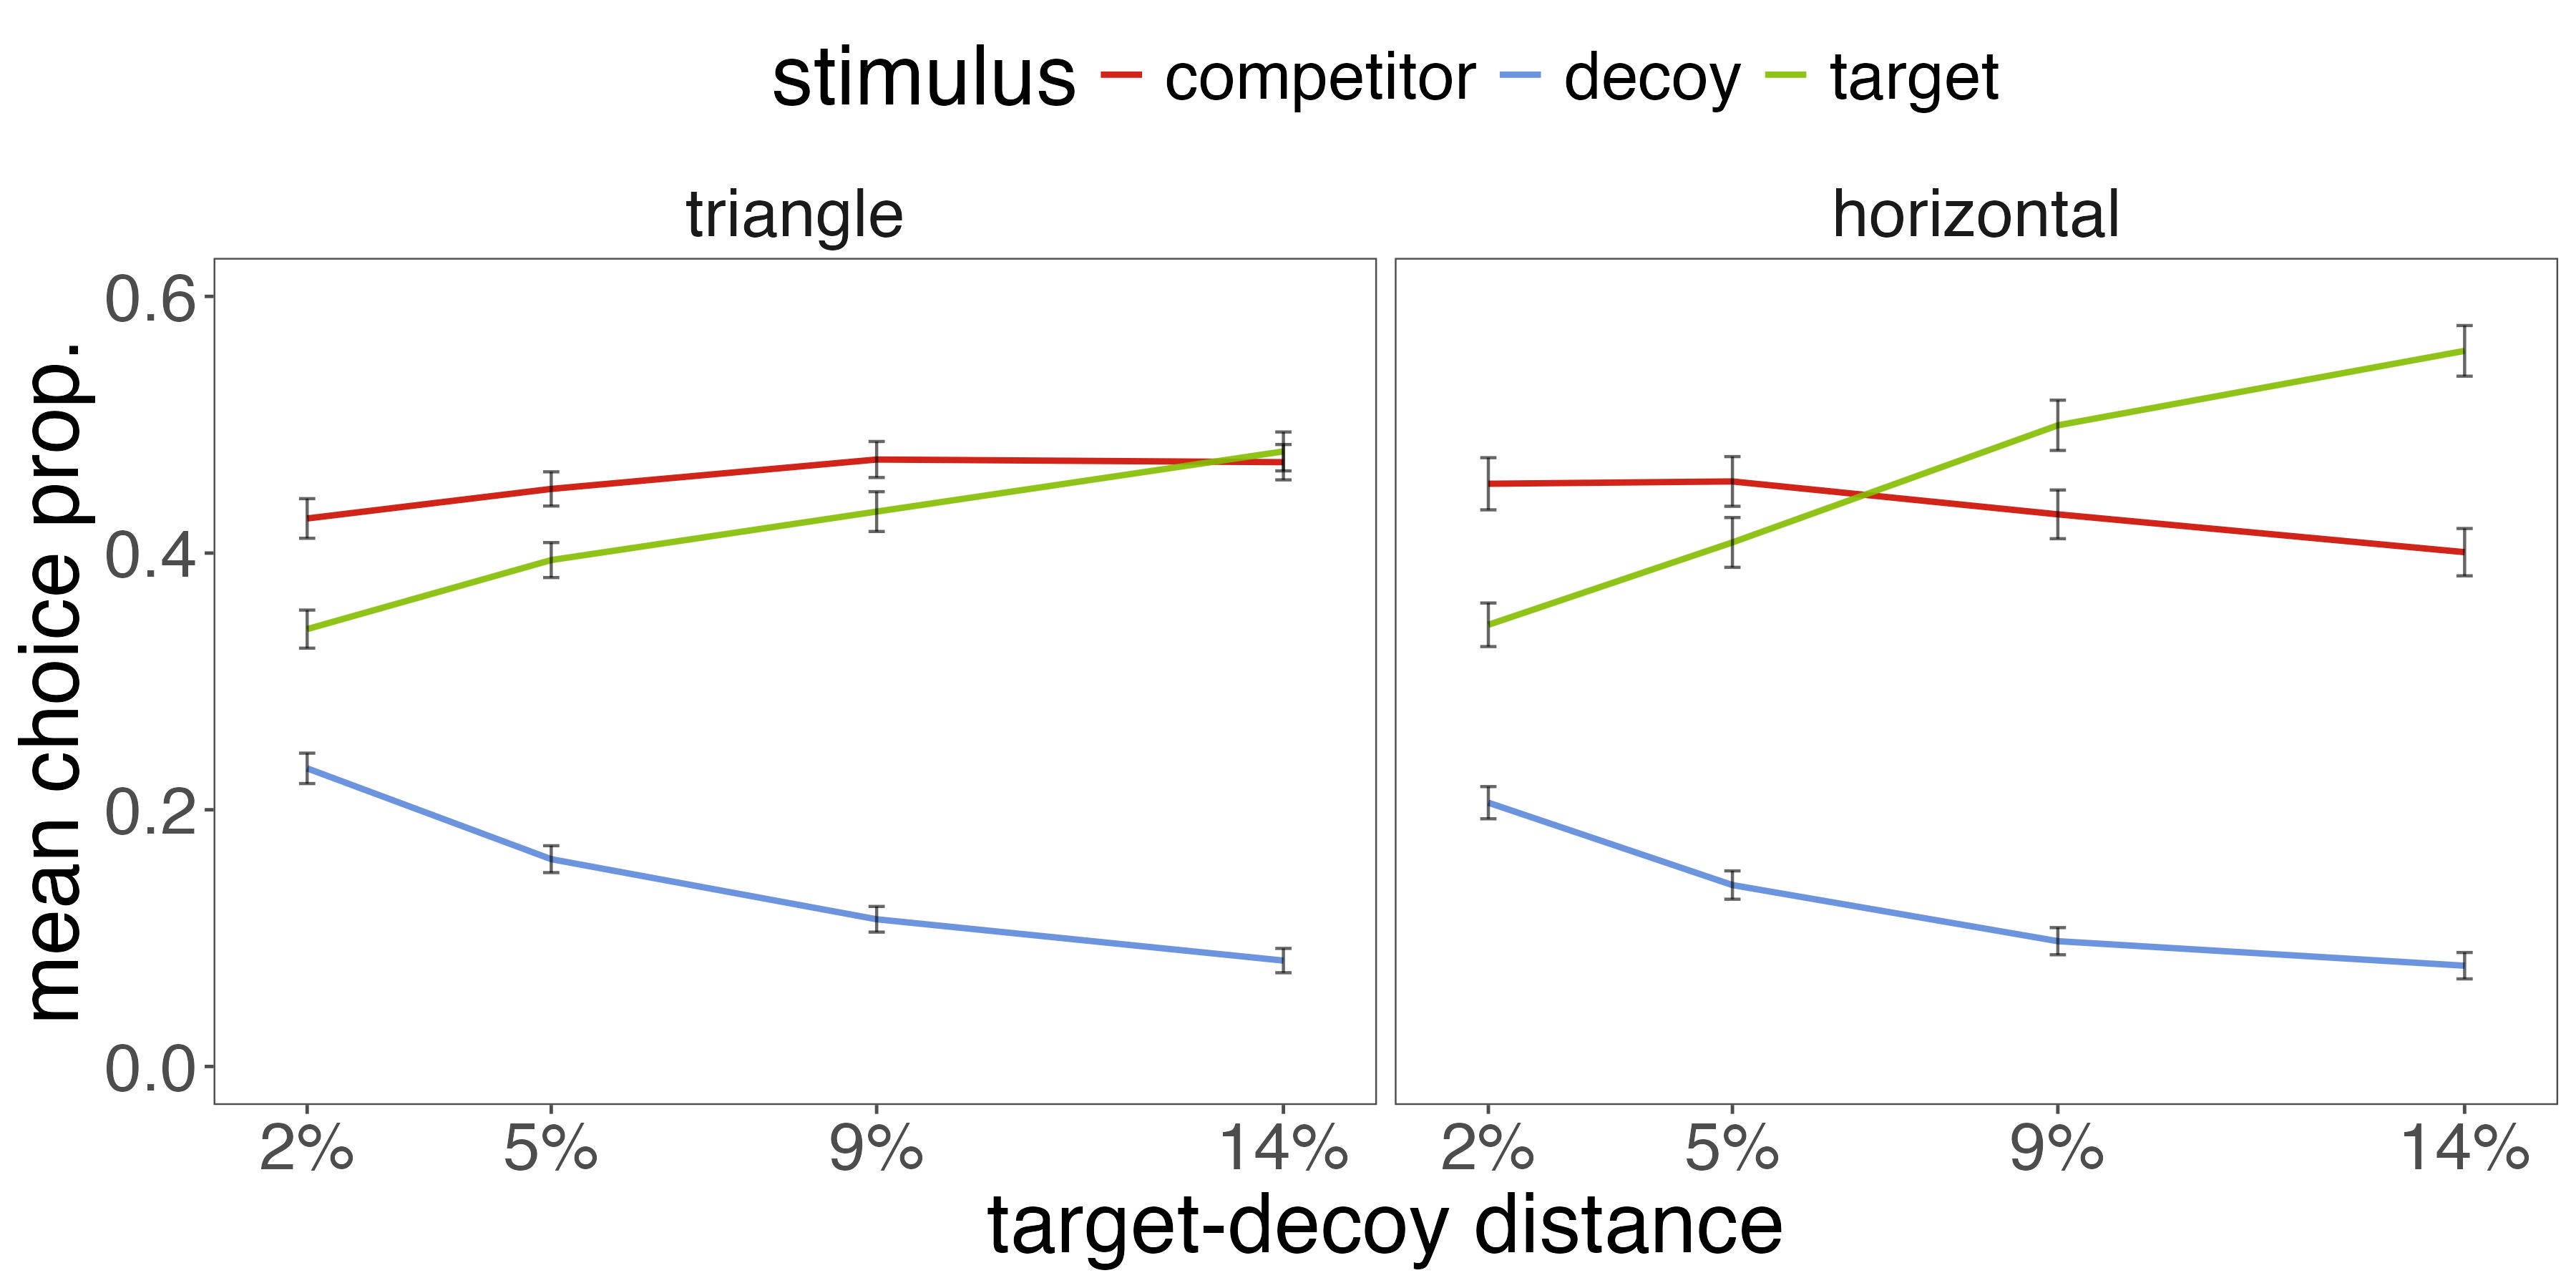
\includegraphics[width=\textwidth]{figures/choicePhase_att_trials_mean_choice_props_collapsed.jpg}
   \caption{Mean choice proportions for target, competitor, and decoy options, by TDD and display condition. THIS FIGURE IS A PLACEHOLDER. WILL CHANGE WITH HDIs FROM STAT. MODEL.}
   \label{fig:e2_choiceprops}
\end{figure}

\begin{figure}
   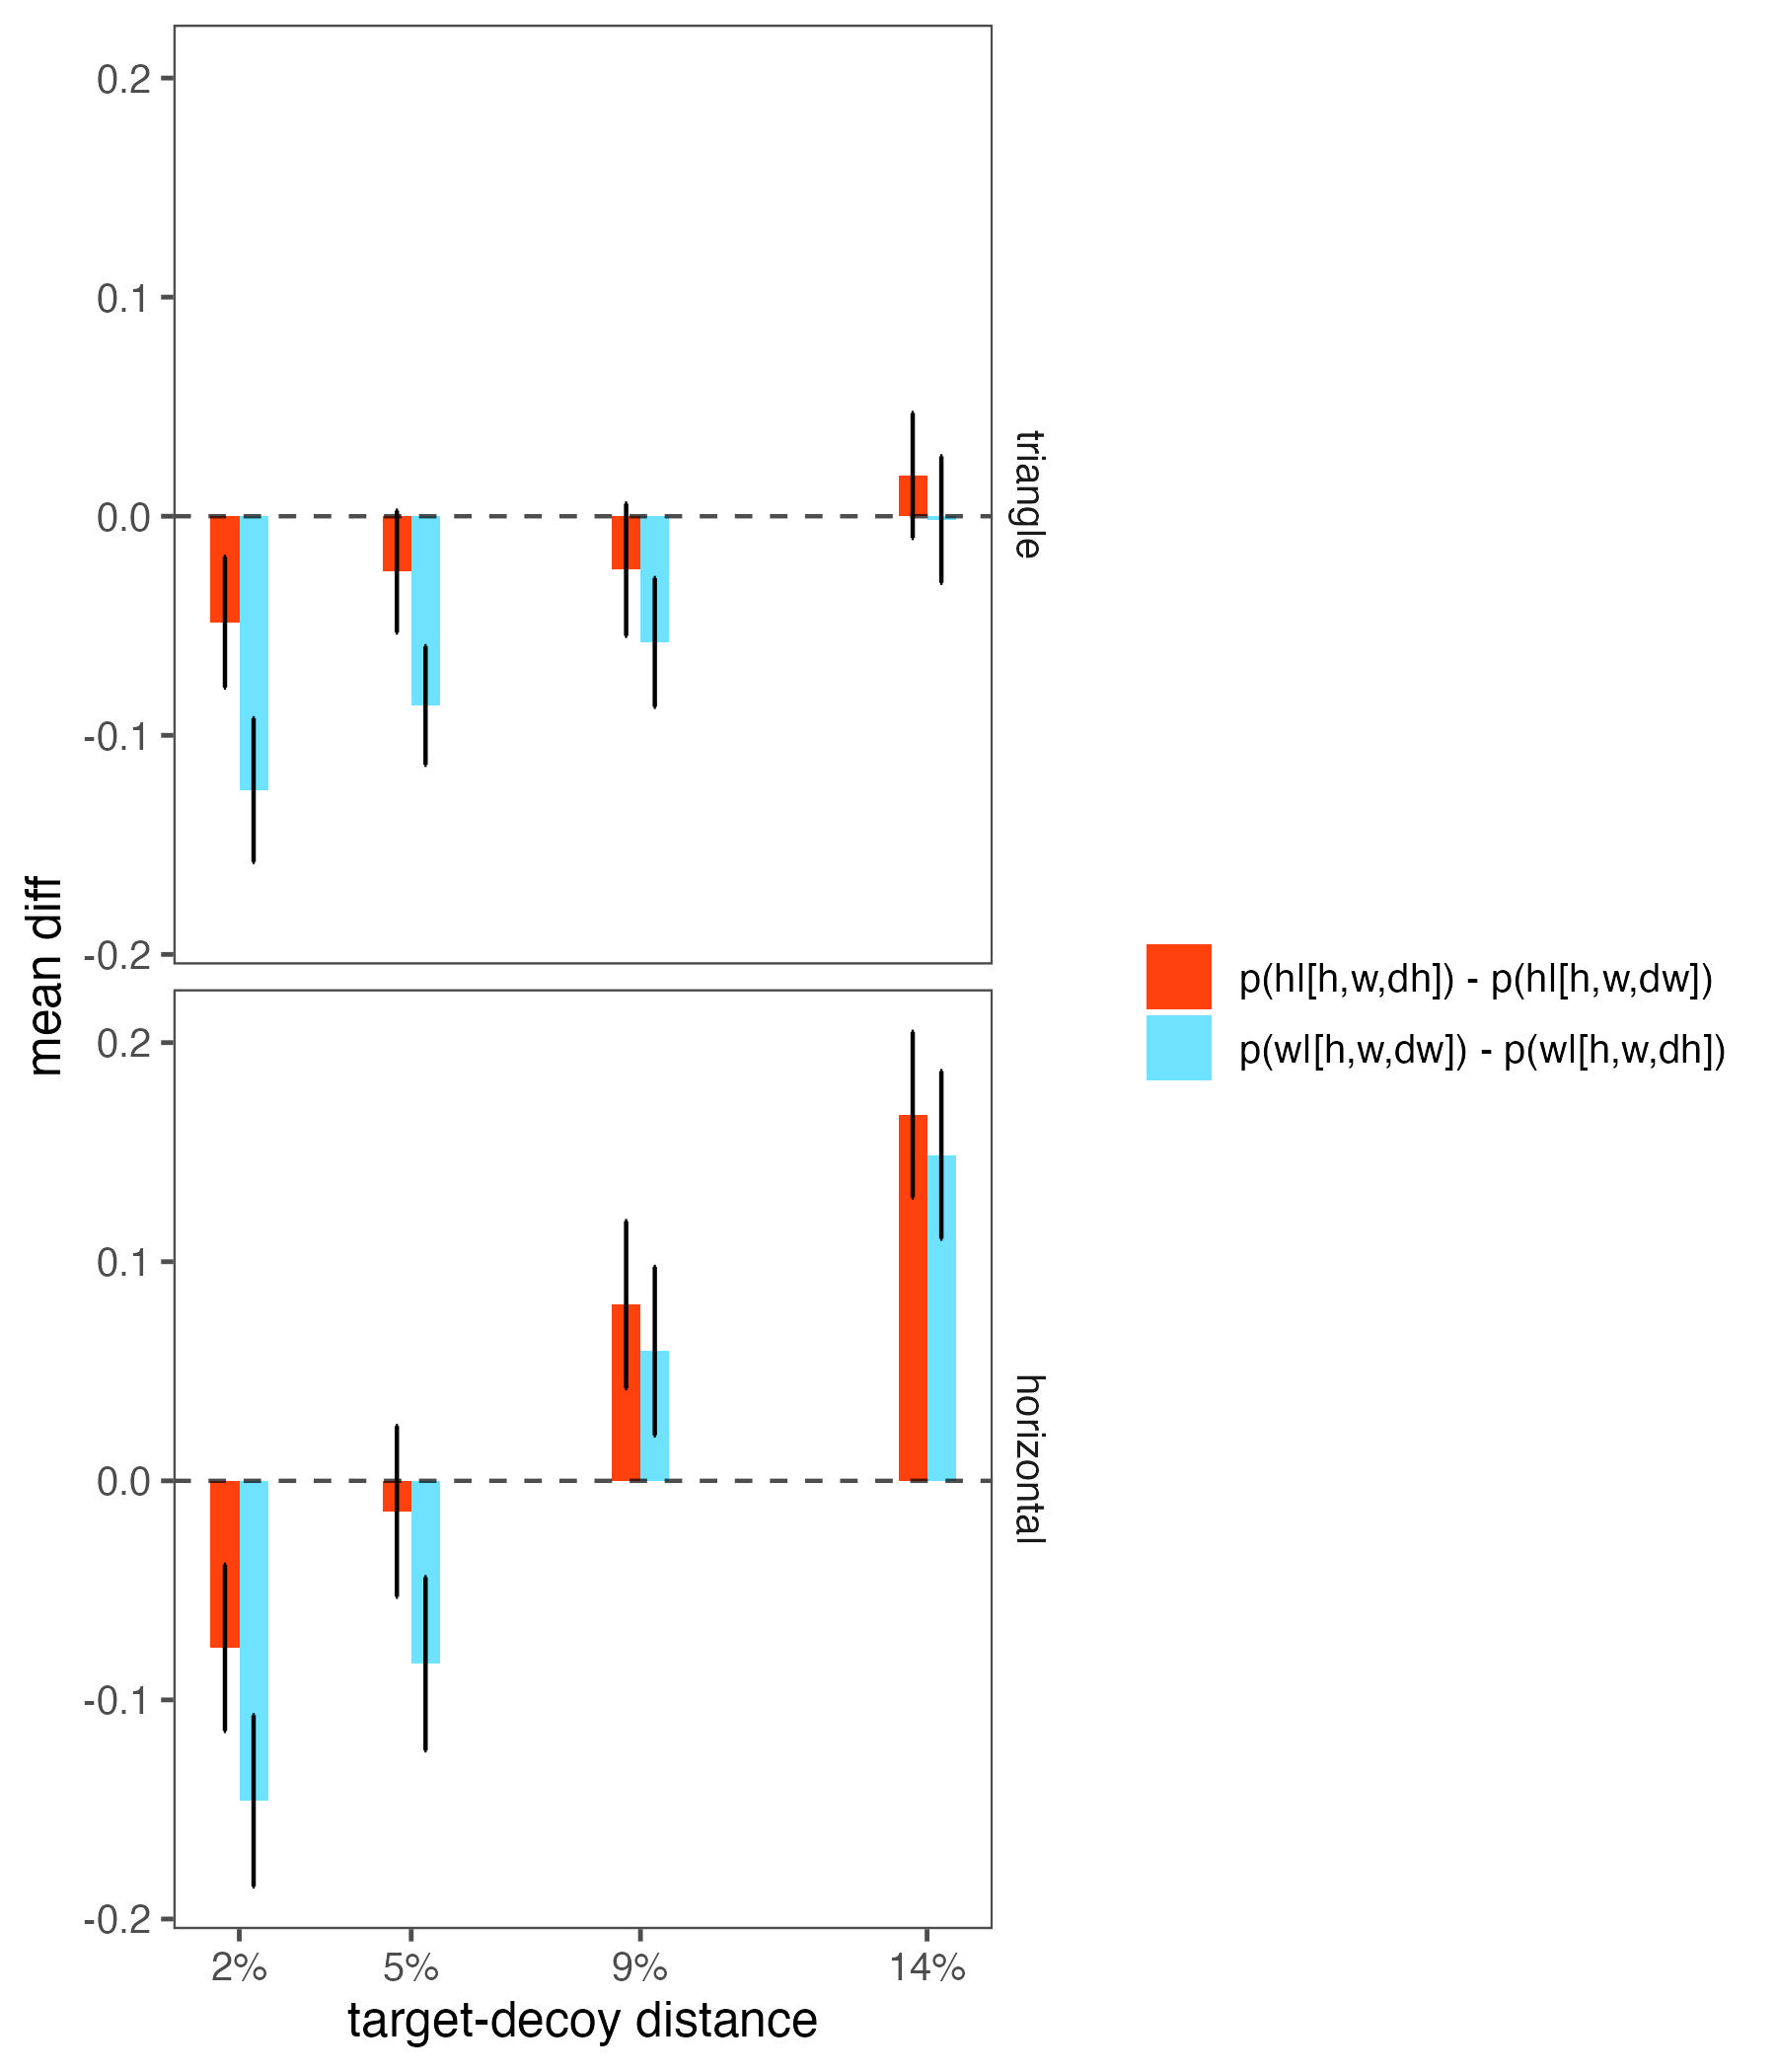
\includegraphics[width=\textwidth]{figures/choicePhase_delta_means.jpeg}
   \caption{Mean changes in choice proportions across choice sets. FIGURE IS ALSO A PLACEHOLDER}
   \label{e2_choicedeltas}
\end{figure}

\subsubsubsection{Model Simulations}
After estimating the parameters of the perceptual model and analyzing the choice data, I sought to test whether the model can predict the choice data. Though I showed in the introduction that this is possible, it was an open question whether the parameters estimated from actual data would produce qualitatively interesting predictions.

I used mean estimates of $\mathbf{\mu}$ and $\mathbf{\Sigma}$ (see Appendix XXX) to generate predictions at each level of TDD in both display conditions. I present the predictions in Figure \ref{fig:e2_model_preds}. 

Given the estimated parameters, the model is able to produce a repulsion effect, but not an attraction effect. This aligns with our predictions from the introduction; the repulsion effect, at least in some forms, can be generated by a higher correlation between target and decoy stimuli compared to target-competitor and competitor-decoy pairs.

\subsection{Discussion}

The results of Experiments 1 and 2 show that participants are not always able to discriminate the decoy from the target and the competitor, and, that target-decoy perceptions appeared to be correlated. The observed correlations can, in turn, naturally produce the repulsion effect but not the attraction effect. 